%%%%%%%%%%%%%%%%%%%%%%%%%%%%%%%%%%%%%%%%%%%%%%%%%%%%%%%%%%%%%%%%%%%%%
%
%  This is a sample LaTeX input file for your contribution to
%  the M&C2019 topical meeting.
%
%  Please use it as a template for your full paper
%    Accompanying/related file(s) include:
%       1. Document class/format file: mandc.cls
%       2. Sample Postscript Figure:   figure.pdf
%       3. A PDF file showing the desired appearance: mandc2019_template.pdf
%       4. cites.sty and citesort.sty that might be needed by some users
%    Direct questions about these files to: palmert@engr.orst.edu
%											mark.dehart@inl.gov
%
%    Notes:
%      (1) You can use the "dvips" utility to convert .dvi
%          files to PostScript.  Then, use either Acrobat
%          Distiller or "ps2pdf" to convert to PDF format.
%      (2) Different versions of LaTeX have been observed to
%          shift the page down, causing improper margins.
%          If this occurs, adjust the "topmargin" value in the
%          physor2018.cls file to achieve the proper margins.
%
%%%%%%%%%%%%%%%%%%%%%%%%%%%%%%%%%%%%%%%%%%%%%%%%%%%%%%%%%%%%%%%%%%%%%


%%%%%%%%%%%%%%%%%%%%%%%%%%%%%%%%%%%%%%%%%%%%%%%%%%%%%%%%%%%%%%%%%%%%%
\documentclass[letterpaper]{mandc2019}
%
%  various packages that you may wish to activate for usage
\usepackage{graphicx} % allows inclusion of graphics
\usepackage{booktabs} % nice rules (thick lines) for tables
\usepackage{microtype} % improves typography for PDF
\usepackage{cleveref}
\usepackage{float}
\usepackage{placeins}
\usepackage{cites}
\usepackage{cite}
\usepackage{epsf}
\usepackage{appendix}
\usepackage{ragged2e}
\usepackage[top=1in, bottom=1.in, left=1.in, right=1.in]{geometry}
\usepackage{enumitem}
\setlist[itemize]{leftmargin=*}
\usepackage{caption}
\captionsetup{width=1.0\textwidth,font={bf,normalsize},skip=0.3cm,within=none,justification=centering}
\usepackage[acronym,toc]{glossaries}
%\newacronym{<++>}{<++>}{<++>}
\newacronym[longplural={metric tons of heavy metal}]{MTHM}{MTHM}{metric ton of heavy metal}
\newacronym{ABM}{ABM}{agent-based modeling}
\newacronym{ACDIS}{ACDIS}{Program in Arms Control \& Domestic and International Security}
\newacronym{AHTR}{AHTR}{Advanced High Temperature Reactor}
\newacronym{ANDRA}{ANDRA}{Agence Nationale pour la gestion des D\'echets RAdioactifs, the French National Agency for Radioactive Waste Management}
\newacronym{ANL}{ANL}{Argonne National Laboratory}
\newacronym{ANS}{ANS}{American Nuclear Society}
\newacronym{API}{API}{application programming interface}
\newacronym{ARE}{ARE}{Aircraft Reactor Experiment}
\newacronym{ARFC}{ARFC}{Advanced Reactors and Fuel Cycles}
\newacronym{ASME}{ASME}{American Society of Mechanical Engineers}
\newacronym{ATWS}{ATWS}{Anticipated Transient Without Scram}
\newacronym{BDBE}{BDBE}{Beyond Design Basis Event}
\newacronym{BIDS}{BIDS}{Berkeley Institute for Data Science}
\newacronym{CAFCA}{CAFCA}{ Code for Advanced Fuel Cycles Assessment }
\newacronym{CDTN}{CDTN}{Centro de Desenvolvimento da Tecnologia Nuclear}
\newacronym{CFD}{CFD}{Computational Fluid Dynamics}
\newacronym{CEA}{CEA}{Commissariat \`a l'\'Energie Atomique et aux \'Energies Alternatives}
\newacronym{CI}{CI}{continuous integration}
\newacronym{CNEN}{CNEN}{Comiss\~{a}o Nacional de Energia Nuclear}
\newacronym{CNERG}{CNERG}{Computational Nuclear Engineering Research Group}
\newacronym{COSI}{COSI}{Commelini-Sicard}
\newacronym{COTS}{COTS}{commercial, off-the-shelf}
\newacronym{CR}{CR}{conversion ratio}
\newacronym{CSNF}{CSNF}{commercial spent nuclear fuel}
\newacronym{CTAH}{CTAHs}{Coiled Tube Air Heaters}
\newacronym{CUBIT}{CUBIT}{CUBIT Geometry and Mesh Generation Toolkit}
\newacronym{CURIE}{CURIE}{Centralized Used Fuel Resource for Information Exchange}
\newacronym{DAG}{DAG}{directed acyclic graph}
\newacronym{DANESS}{DANESS}{Dynamic Analysis of Nuclear Energy System Strategies}
\newacronym{DBE}{DBE}{Design Basis Event}
\newacronym{DESAE}{DESAE}{Dynamic Analysis of Nuclear Energy Systems Strategies}
\newacronym{DHS}{DHS}{Department of Homeland Security}
\newacronym{DOE}{DOE}{Department of Energy}
\newacronym{DRACS}{DRACS}{Direct Reactor Auxiliary Cooling System}
\newacronym{DRE}{DRE}{dynamic resource exchange}
\newacronym{DSNF}{DSNF}{DOE spent nuclear fuel}
\newacronym{DU}{DU}{depleted uranium}
\newacronym{DYMOND}{DYMOND}{Dynamic Model of Nuclear Development }
\newacronym{EBS}{EBS}{Engineered Barrier System}
\newacronym{EDF}{EDF}{Électricité de France}
\newacronym{EDZ}{EDZ}{Excavation Disturbed Zone}
\newacronym{EIA}{EIA}{U.S. Energy Information Administration}
\newacronym{EPA}{EPA}{Environmental Protection Agency}
\newacronym{EPR}{EPR}{European Pressurized Reactors}
\newacronym{EP}{EP}{Engineering Physics}
\newacronym{EU}{EU}{European Union}
\newacronym{FCO}{FCO}{Fuel Cycle Options}
\newacronym{FCT}{FCT}{Fuel Cycle Technology}
\newacronym{FEHM}{FEHM}{Finite Element Heat and Mass Transfer}
\newacronym{FEPs}{FEPs}{Features, Events, and Processes}
\newacronym{FHR}{FHR}{Fluoride-Salt-Cooled High-Temperature Reactor}
\newacronym{FLiBe}{FLiBe}{Fluoride-Lithium-Beryllium}
\newacronym{FP}{FP}{Fission Product}
\newacronym{GDSE}{GDSE}{Generic Disposal System Environment}
\newacronym{GDSM}{GDSM}{Generic Disposal System Model}
\newacronym{GENIUSv1}{GENIUSv1}{Global Evaluation of Nuclear Infrastructure Utilization Scenarios, Version 1}
\newacronym{GENIUSv2}{GENIUSv2}{Global Evaluation of Nuclear Infrastructure Utilization Scenarios, Version 2}
\newacronym{GENIUS}{GENIUS}{Global Evaluation of Nuclear Infrastructure Utilization Scenarios}
\newacronym{GIF}{GIF}{Generation IV International Forum}
\newacronym{GPAM}{GPAM}{Generic Performance Assessment Model}
\newacronym{GRSAC}{GRSAC}{Graphite Reactor Severe Accident Code}
\newacronym{GUI}{GUI}{graphical user interface}
\newacronym{HLW}{HLW}{high level waste}
\newacronym{HPC}{HPC}{high-performance computing}
\newacronym{HTC}{HTC}{high-throughput computing}
\newacronym{HTGR}{HTGR}{High Temperature Gas-Cooled Reactor}
\newacronym{IAEA}{IAEA}{International Atomic Energy Agency}
\newacronym{IEMA}{IEMA}{Illinois Emergency Mangament Agency}
\newacronym{IHLRWM}{IHLRWM}{International High Level Radioactive Waste Management}
\newacronym{INL}{INL}{Idaho National Laboratory}
\newacronym{IPRR1}{IRP-R1}{Instituto de Pesquisas Radioativas Reator 1}
\newacronym{IRP}{IRP}{Integrated Research Project}
\newacronym{ISFSI}{ISFSI}{Independent Spent Fuel Storage Installation}
\newacronym{ISRG}{ISRG}{Independent Student Research Group}
\newacronym{JFNK}{JFNK}{Jacobian-Free Newton Krylov}
\newacronym{LANL}{LANL}{Los Alamos National Laboratory}
\newacronym{LBNL}{LBNL}{Lawrence Berkeley National Laboratory}
\newacronym{LCOE}{LCOE}{levelized cost of electricity}
\newacronym{LDRD}{LDRD}{laboratory directed research and development}
\newacronym{LFR}{LFR}{Lead-Cooled Fast Reactor}
\newacronym{LLNL}{LLNL}{Lawrence Livermore National Laboratory}
\newacronym{LMFBR}{LMFBR}{Liquid Metal Fast Breeder Reactor}
\newacronym{LOFC}{LOFC}{Loss of Forced Cooling}
\newacronym{LOHS}{LOHS}{Loss of Heat Sink}
\newacronym{LOLA}{LOLA}{Loss of Large Area}
\newacronym{LP}{LP}{linear program}
\newacronym{LWR}{LWR}{light water reactor}
\newacronym{MAGNOX}{MAGNOX}{Magnesium Alloy Graphie Moderated Gas Cooled Uranium Oxide Reactor}
\newacronym{MA}{MA}{minor actinide}
\newacronym{MCNP}{MCNP}{Monte Carlo N-Particle code}
\newacronym{MILP}{MILP}{mixed-integer linear program}
\newacronym{MIT}{MIT}{the Massachusetts Institute of Technology}
\newacronym{MOAB}{MOAB}{Mesh-Oriented datABase}
\newacronym{MOOSE}{MOOSE}{Multiphysics Object-Oriented Simulation Environment}
\newacronym{MOSART}{MOSART}{Molten Salt Actinide Recycler and Transmuter}
\newacronym{MOX}{MOX}{mixed oxide}
\newacronym{MPI}{MPI}{Message Passing Interface}
\newacronym{MCSFR}{MCSFR}{Molten Chloride Salt Fast Reactor}
\newacronym{MSBR}{MSBR}{Molten Salt Breeder Reactor}
\newacronym{MSFR}{MSFR}{Molten Salt Fast Reactor}
\newacronym{MSRE}{MSRE}{Molten Salt Reactor Experiment}
\newacronym{MSR}{MSR}{Molten Salt Reactor}
\newacronym{MT}{MT}{metric ton}
\newacronym{NAGRA}{NAGRA}{National Cooperative for the Disposal of Radioactive Waste}
\newacronym{NEAMS}{NEAMS}{Nuclear Engineering Advanced Modeling and Simulation}
\newacronym{NEUP}{NEUP}{Nuclear Energy University Programs}
\newacronym{NFCSim}{NFCSim}{Nuclear Fuel Cycle Simulator}
\newacronym{NGNP}{NGNP}{Next Generation Nuclear Plant}
\newacronym{NMWPC}{NMWPC}{Nuclear MW Per Capita}
\newacronym{NNSA}{NNSA}{National Nuclear Security Administration}
\newacronym{NPP}{NPP}{Nuclear Power Plant}
\newacronym{NPRE}{NPRE}{Department of Nuclear, Plasma, and Radiological Engineering}
\newacronym{NQA1}{NQA-1}{Nuclear Quality Assurance - 1}
\newacronym{NRC}{NRC}{Nuclear Regulatory Commission}
\newacronym{NSF}{NSF}{National Science Foundation}
\newacronym{NSSC}{NSSC}{Nuclear Science and Security Consortium}
\newacronym{NUWASTE}{NUWASTE}{Nuclear Waste Assessment System for Technical Evaluation}
\newacronym{NWF}{NWF}{Nuclear Waste Fund}
\newacronym{NWTRB}{NWTRB}{Nuclear Waste Technical Review Board}
\newacronym{OCRWM}{OCRWM}{Office of Civilian Radioactive Waste Management}
\newacronym{ORION}{ORION}{ORION}
\newacronym{ORNL}{ORNL}{Oak Ridge National Laboratory}
\newacronym{PARCS}{PARCS}{Purdue Advanced Reactor Core Simulator}
\newacronym{PBAHTR}{PB-AHTR}{Pebble Bed Advanced High Temperature Reactor}
\newacronym{PBFHR}{PB-FHR}{Pebble-Bed Fluoride-Salt-Cooled High-Temperature Reactor}
\newacronym{PEI}{PEI}{Peak Environmental Impact}
\newacronym{PH}{PRONGHORN}{PRONGHORN}
\newacronym{PRIS}{PRIS}{Power Reactor Information System}
\newacronym{PRKE}{PRKE}{Point Reactor Kinetics Equations}
\newacronym{PSPG}{PSPG}{Pressure-Stabilizing/Petrov-Galerkin}
\newacronym{PWAR}{PWAR}{Pratt and Whitney Aircraft Reactor}
\newacronym{PWR}{PWR}{Pressurized Water Reactor}
\newacronym{PyNE}{PyNE}{Python toolkit for Nuclear Engineering}
\newacronym{PyRK}{PyRK}{Python for Reactor Kinetics}
\newacronym{QA}{QA}{quality assurance}
\newacronym{RDD}{RD\&D}{Research Development and Demonstration}
\newacronym{RD}{R\&D}{Research and Development}
\newacronym{REE}{REE}{rare earth element}
\newacronym{RELAP}{RELAP}{Reactor Excursion and Leak Analysis Program}
\newacronym{RIA}{RIA}{Reactivity Insertion Accident}
\newacronym{RIF}{RIF}{Region-Institution-Facility}
\newacronym{RTh}{RTh}{recovered thorium}
\newacronym{RU}{RU}{recovered uranium}
\newacronym{SFR}{SFR}{Sodium-Cooled Fast Reactor}
\newacronym{SINDAG}{SINDA{\textbackslash}G}{Systems Improved Numerical Differencing Analyzer $\backslash$ Gaski}
\newacronym{SKB}{SKB}{Svensk K\"{a}rnbr\"{a}nslehantering AB}
\newacronym{SNF}{SNF}{spent nuclear fuel}
\newacronym{SNL}{SNL}{Sandia National Laboratory}
\newacronym{STC}{STC}{specific temperature change}
\newacronym{SUPG}{SUPG}{Streamline-Upwind/Petrov-Galerkin}
\newacronym{SWF}{SWF}{Separations and Waste Forms}
\newacronym{SWU}{SWU}{Separative Work Unit}
\newacronym{TRIGA}{TRIGA}{Training Research Isotope General Atomic}
\newacronym{TRISO}{TRISO}{Tristructural Isotropic}
\newacronym{TRU}{TRU}{transuranic}
\newacronym{TSM}{TSM}{Total System Model}
\newacronym{TSPA}{TSPA}{Total System Performance Assessment for the Yucca Mountain License Application}
\newacronym{ThOX}{ThOX}{thorium oxide}
\newacronym{UFD}{UFD}{Used Fuel Disposition}
\newacronym{UML}{UML}{Unified Modeling Language}
\newacronym{UOX}{UOX}{uranium oxide}
\newacronym{UQ}{UQ}{uncertainty quantification}
\newacronym{US}{US}{United States}
\newacronym{UW}{UW}{University of Wisconsin}
\newacronym{VISION}{VISION}{the Verifiable Fuel Cycle Simulation Model}
\newacronym{VVER}{VVER}{Voda-Vodyanoi Energetichesky Reaktor (Russian Pressurized Water Reactor)}
\newacronym{VV}{V\&V}{verification and validation}
\newacronym{WIPP}{WIPP}{Waste Isolation Pilot Plant}
\newacronym{YMR}{YMR}{Yucca Mountain Repository Site}


\makeglossaries
%\usepackage[justification=centering]{caption}

%
% Define title...
%
\title{FUEL CYCLE PERFORMANCE OF FAST SPECTRUM \\
  MOLTEN SALT REACTOR DESIGNS
\footnote{Notice:  This manuscript has been authored by UT-Battelle, LLC, under contract DE-AC05-00OR22725 with the US Department of Energy (DOE). The US government retains and the publisher, by accepting the article for publication, acknowledges that the US government retains a nonexclusive, paid-up, irrevocable, worldwide license to publish or reproduce the published form of this manuscript, or allow others to do so, for US government purposes. DOE will provide public access to these results of federally sponsored research in accordance with the DOE Public Access Plan (http://energy.gov/downloads/doe-public-access-plan).}
		}
%
% ...and authors
%

\author{%
  % FIRST AUTHORS
  %
  \textbf{Andrei Rykhlevskii$^1$, Benjamin R. Betzler$^2$, Andrew Worrall$^2$, and Kathryn Huff$^1$} \\
  $^1$Dept. of Nuclear, Plasma, and Radiological Engineering, University of Illinois at \\
  Urbana-Champaign, Urbana, IL 61801 \\
\\
  $^2$Oak Ridge National Laboratory \\
1 Bethel Valley Road, Oak Ridge, TN, USA  \\
\\
  \url{andreir2@illinois.edu}, \url{betzlerbr@ornl.gov}, \url{worralla@ornl.gov}, \url{kdhuff@illinois.edu}
}
%
% Insert authors' names and short version of title in lines below
%
\newcommand{\authorHead}      % Author's names here use et al. if more than 3
           {Andrei Rykhlevskii et al.}
\newcommand{\shortTitle}      % Short title here (Shorten to fit all into a single line)
           {Fuel Cycle Performance of Fast Molten Salt Reactor designs}
%%%%%%%%%%%%%%%%%%%%%%%%%%%%%%%%%%%%%%%%%%%%%%%%%%%%%%%%%%%%%%%%%%%%%
%
%   BEGIN DOCUMENT
%
%%%%%%%%%%%%%%%%%%%%%%%%%%%%%%%%%%%%%%%%%%%%%%%%%%%%%%%%%%%%%%%%%%%%%
\begin{document}
\maketitle
\justify

\begin{abstract}
In the search for new ways to generate carbon-free, reliable 
base-load power, interest in advanced nuclear energy technologies, 
particularly \glspl{MSR}, has resurged with multiple new conceptual \glspl{MSR} including fast neutron spectrum designs. The fuel cycle performance of four perspective fast \gls{MSR} designs is analyzed using a recently developed SCALE/TRITON 6.2.4 Alpha with continuous online reprocessing support. The fast spectrum and continuous feeds/removals enable these concepts to have remarkable fuel  cycle metrics: (1) resource utilization is about 18 times better than for typical light water reactor (i.e., from $\sim180$ t/GWe-yr to $\sim1$ t/GWe-yr); (2) fast \glspl{MSR} generate about 25 times less nuclear waste than light water reactors. These metrics are compared to similar fuel cycles using alternative technologies. Additionally, full-core and unit cell transport models were created and compared to prove the viability of using simplified unit cell geometries for long-term depletion simulation. The unit cell approximation provided a 20x speedup when depleted mass relative error for major isotopes is less than 2\%. Additional fast \glspl{MSR} design and analysis challenges associated with different fuel cycles and the use of molten salt reactor technology are addressed and discussed.
\end{abstract}
\keywords{molten salt reactor, fast reactor, depletion, fuel cycle, salt treatment, salt separations}

%%%%%%%%%%%%%%%%%%%%%%%%%%%%%%%%%%%%%%%%%%%%%%%%%%%%%%%%%%%%%%%%%%%%%%%%%%%%%%%%
\section{INTRODUCTION}
\label{sec:intro}
Liquid-fueled \gls{MSR} concepts are one of many advanced reactor technologies that promise a competitive and sustainable energy source \cite{siemer_why_2015}. In these \gls{MSR}s, fissile and/or fertile materials are dissolved in a carrier molten salt (e.g., LiF or NaCl), which offers for several advantages over solid-fueled reactors. These include near-atmospheric pressure in the primary loop, relatively high coolant temperature, outstanding neutron economy, a high level of inherent safety,
reduced fuel preprocessing, and the ability to continuously remove fission products and add fissile and/or fertile elements without shutdown \cite{leblanc_molten_2010}.

Historically, operational experience was limited to thermal spectrum \gls{MSR} concepts with a solid graphite moderator.  \gls{ORNL} operated an $\approx$8 MW$_{th}$ \gls{MSRE} from 1965 to 1969 to test approaches and materials, demonstrate fissile recycle (both $^{233}$U and $^{235}$U), and determine generic \gls{MSR} operational characteristics \cite{macpherson_molten_1985}. Experience and promising breakthroughs in reprocessing technologies \cite{whatley_engineering_1970} led \gls{ORNL} to the simply configured, graphite-moderated (i.e., thermal or intermediate spectrum), single-fluid \gls{MSBR} by the end of the 1960's. The primary weakness of these single-fluid thermal \gls{MSR} concepts is that the hundreds of tons ($\approx$300 t for \gls{MSBR} \cite{robertson_conceptual_1971}) of expensive, radiologically contaminated, and irradiated graphite require replacement every 4--10 years, raising significant waste and economical issues.

In contrast, consistent with \gls{GIF} sustainability and safety goals \cite{gif_generation_2015}, unmoderated (no graphite), one- or two-fluid (blanket-equipped) fast spectrum \gls{MSR} concepts eventually became the Euratom ``reference'' \gls{MSR} \cite{euratom_final_2015}. Fast \gls{MSR} systems hold additional advantages over conventional \glspl{LWR}:
(1) they can operate as a breeder (i.e., with \gls{CR}\footnote{\gls{CR} $\equiv$ fissile generated/fissile consumed: if CR$<$1, the reactor is a ``converter''; CR$\equiv$1, an ``isobreeder''; CR$>$1, a ``breeder''.}$>$1) \cite{euratom_final_2015, simmons_assessment_1974, mourogov_potentialities_2006-1}, fertile-free \gls{TRU} burner, or U/Th-supported \gls{TRU} burner \cite{ignatiev_progress_2007};
(2) they have the potential to be used in both $^{232}$Th/$^{233}$U and $^{238}$U/$^{239}$Pu fuel cycles;
(3) they can be operated in ways that would generate very little long-lived \gls{TRU} waste; and
(4) they would use reduced amounts of natural resources (e.g., natural uranium, natural thorium) per unit energy generated. To quantitatively estimate the benefits of these capabilities, a fuel cycle performance analysis for various fast spectrum \gls{MSR} concepts is necessary.

Much of the analysis herein uses unit cell representations of four different fast \gls{MSR} designs:
(1) European \gls{MSFR} \cite{euratom_final_2015};
(2) \gls{MCSFR} \cite{simmons_assessment_1974};
(3) REBUS-3700 \cite{mourogov_potentialities_2006-1};
(4) \gls{MOSART} \cite{ignatiev_progress_2007}.
Some of these designs are two fluid (1, 2), operate in thorium fuel cycle (1,4), or use \gls{TRU} as start-up fissile material (3, 4). Concepts (2) and (3) use chloride salts,\footnote{The chlorine in the \gls{MCSFR} is fully enriched in $^{37}$Cl because $^{35}$Cl (76\% abundance) is a very strong neutron poison in the fast-neutron energy range.} while (1) and (4) use fluorides. This paper discusses the fuel cycle simulation of these concepts to quantify the fuel cycle performance of fast \glspl{MSR}.
\section{METHODS}
\label{sec:methods}
Full-core and simplified unit cell models of four different fast spectrum \glspl{MSR} designs are created (Fig.~\ref{fig:unit_cell}) to determine fuel cycle performance parameters. For full-core models realistic vacuum boundary conditions were applied  while unit cell simplified models used reflective boundary conditions which do not take into account neutron leakage (infinite reactor was assumed). Table~\ref{table:fsmsr_concepts} contains a summary of the principal data of these designs. Fuel cycle performance analysis requires a depletion simulation for each reactor concept over the system lifetime, which in this work is assumed to be 60 years\footnote{The lifetime of a fast \gls{MSR} is limited by neutron damage on the reactor vessel. Further R\&D activities should be performed to evaluate the maximum fast-neutron fluence and assess structural materials choice.}. Full-core 60-year depletion calculations for \gls{MSR}s are computationally prohibitive. Computation time can be significantly reduced by performing depletion simulations for representative simplified unit cells instead of complex full-core geometry.
\begin{figure}[!htb]
  \centering
    \vspace{-0.2in}
  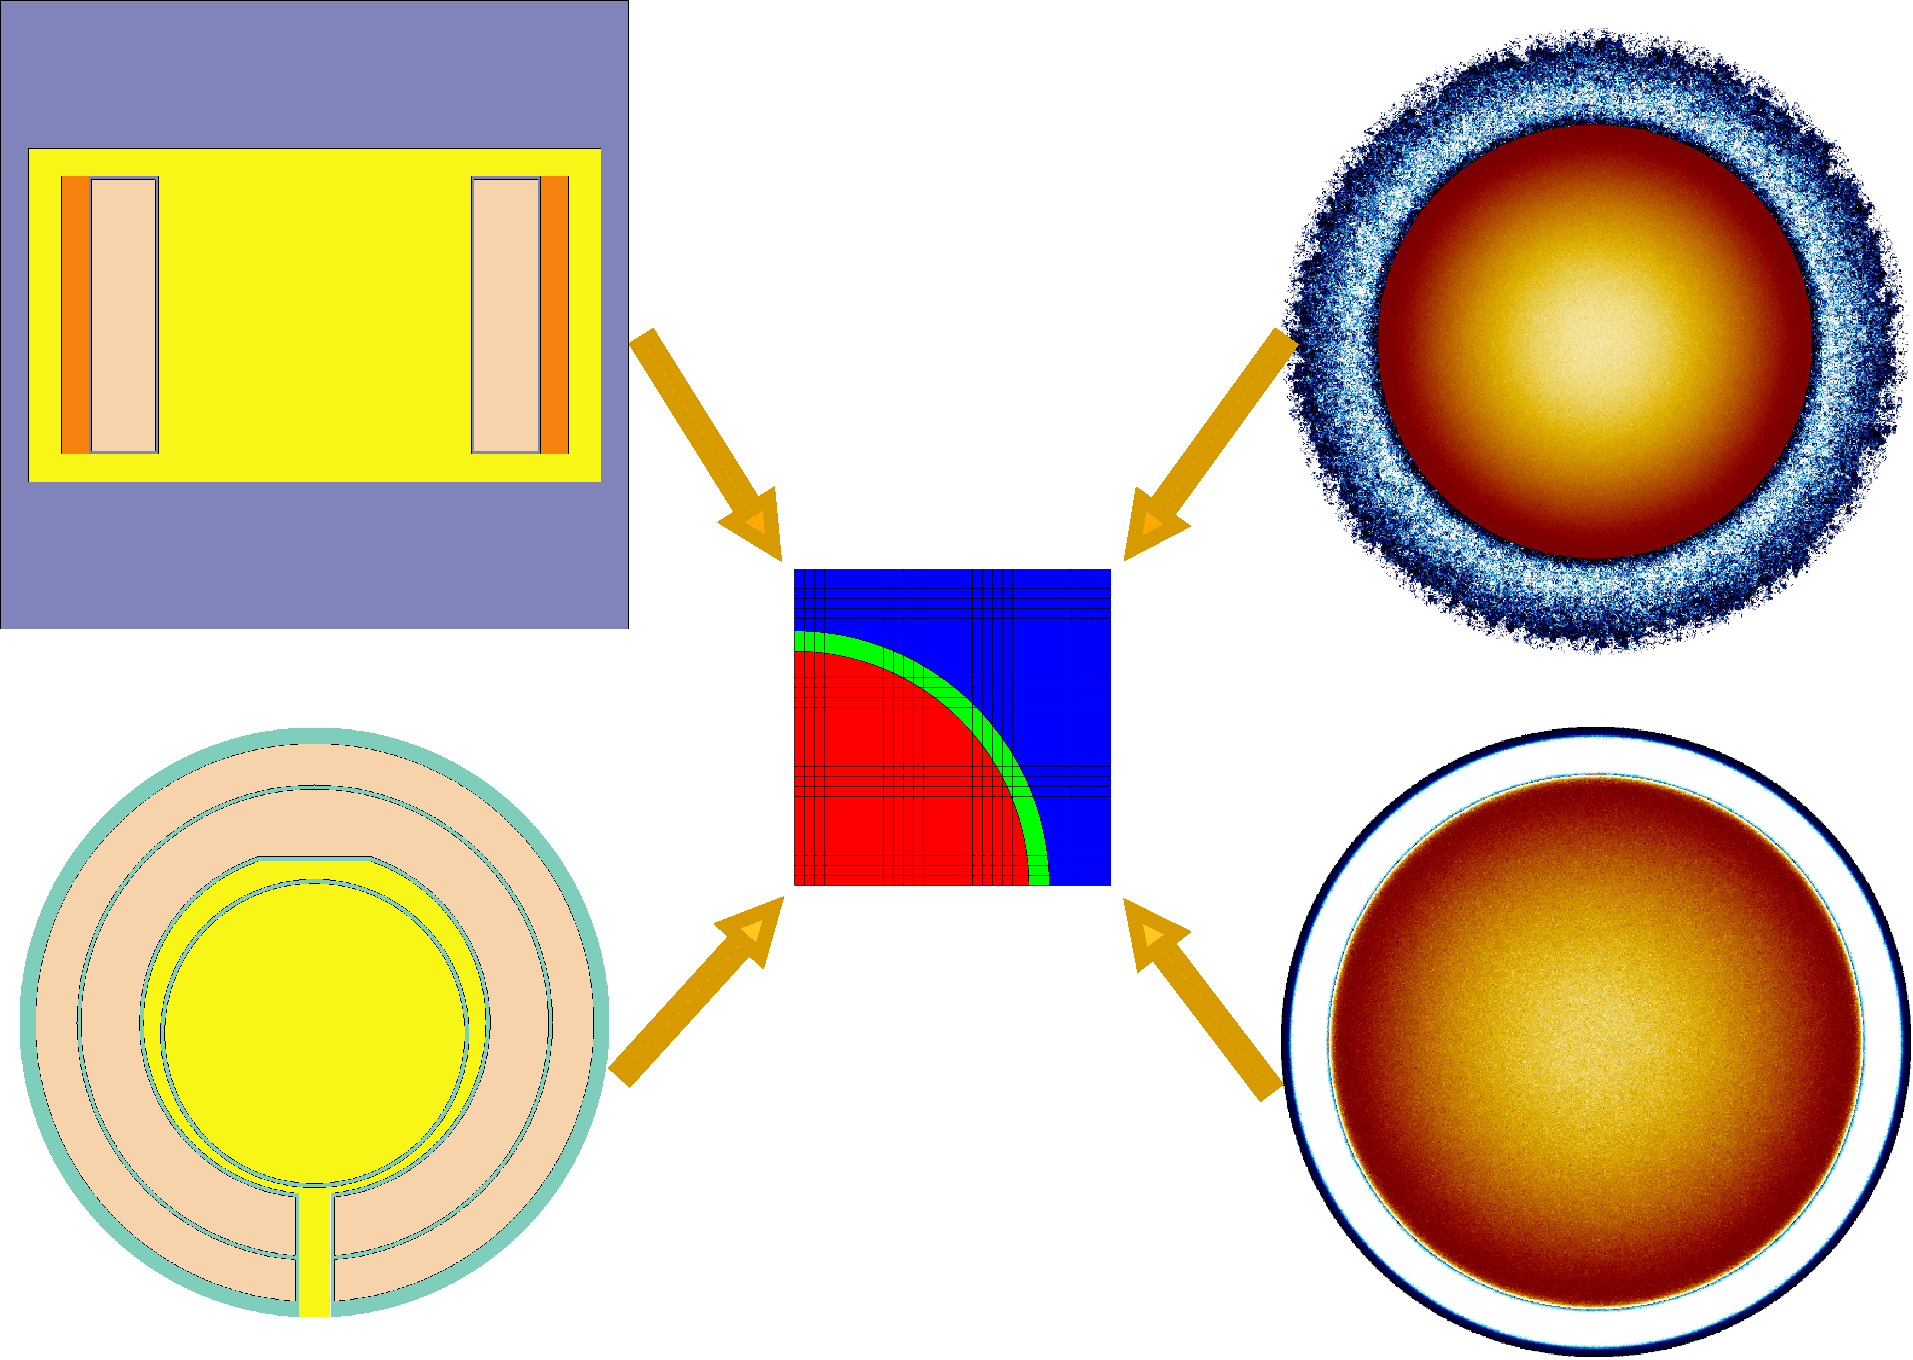
\includegraphics[width=0.8\textwidth]{./Figures/fsmsrs.pdf}
  \caption{Full-core 3D models of \gls{MSFR} (upper left), \gls{MCSFR} (lower left), REBUS-3700 (upper right), \gls{MOSART} (lower right), and 2D representative unit cell model (center) showing fuel salt (red), fertile salt (green), structural material (blue).}
  \label{fig:unit_cell}
  \vspace{-0.5in}
\end{figure}
\subsection{Tool description}
All salt treatments and separation in this work are performed as truly continuous (online) processes using SCALE/TRITON version 6.2.4 Alpha \cite{betzler_implementation_2017-1} with the 238-group ENDF-B/VII.1 cross-section library \cite{rearden_scale_2016}. Several earlier studies used a batch-wise approach because most reactor physics depletion tools are designed to model batch-fueled reactors with solid fuel \cite{betzler_molten_2017,rykhlevskii_online_2017,rykhlevskii_modeling_2019}. This approach requires short depletion time steps to minimize the impact of material feeds and removals during a given time step, leading to a large number of depletion time steps (i.e., transport calculations). This makes lifetime-long depletion calculations computationally expensive. ORIGEN \cite{gauld_isotopic_2011} supports continuous feeds and removals but does not track the feed and discharge materials that are important to fuel cycle performance analysis. Thus, the version of SCALE/TRITON currently under testing at \gls{ORNL} enables the simulation of continuous processes and the tracking of removed materials over the \gls{MSR} lifetime at a reasonable computational cost. \par
SCALE/TRITON Alpha currently supports only constant or piece-wise feed and removal rates. Therefore, these rates must be determined for each feed and removal before running a simulation and cannot be adjusted during simulation. One of the features of fast spectrum \gls{MSR}s is the control of long-term reactivity through the fertile material feed rate, avoiding the use of classic reactivity control devices (e.g., reactivity control rods, burnable poisons, soluble poisons). Overall, reactivity control for fast spectrum \gls{MSR}s presents an engineering challenge and is outside of the scope of the paper. Another feature of \gls{MSR}s, delayed neutron precursor drift corresponding to its circulating liquid fuel, is very important for safety transient analysis but has a negligible effect on long-term depletion calculations and  not treated here. 
\begin{table*}[!htb]
\vspace{-0.3in}
  \centering
  \caption{Principal data of selected fast spectrum \gls{MSR} designs.}
  \label{table:fsmsr_concepts}
  \begin{tabular}{p{0.27\textwidth} p{0.14\textwidth} p{0.14\textwidth} p{0.18\textwidth} p{0.14\textwidth}} \toprule
   Parameter & \gls{MSFR} & \gls{MCSFR} & REBUS-3700 & \gls{MOSART} \\ \midrule
   Thermal power, MW 				&  3,000 & 6,000     & 3,700 & 2,400   \\
   Fuel salt volume (in/out), m$^3$       &18 (9/9)& 38 (16/22)& 55.6 (36.9/18.7) & 49.05 (32.7/16.35) \\
   Fertile salt volume (in/out), m$^3$ & 7.3 (7.3/0) & 75 (55/22)    & --- & --- \\
   Fuel and fertile salt initial composition, mol\% & LiF-ThF$_4$-$^{233}$UF$_4$ (77.5-19.9-2.6) LiF-ThF$_4$ \newline (77.5-22.5) & NaCl-UCl$_3$-$^{239}$PuCl$_3$ (60-36-4) \newline NaCl-UCl$_3$ \newline (60-40)
   & 55mol\%NaCl+ 45mol\%(natU+ 16.7at.\%TRU)Cl$_3$
   & LiF-BeF$_2$-ThF$_4$-TRUF$_3$  \newline (69.72-27-1.28) \\
   Fuel cycle & Th/$^{233}$U & U/Pu  & U/TRU & Th/$^{233}$U \\
   Initial fissile inventory, t & \ 7.726 & \ 9.400    & 18.061 & 9.637 \\ \bottomrule
   \end{tabular}
   \vspace{-0.5in}
\end{table*}
\subsection{Models description}
\label{sec:model}
In contrast with thermal \gls{MSR}s, fast spectrum concepts do not have a channel or assembly structure but instead use a cylindrical or spherical vessel to contain the homogenized fuel mixture. Two-fluid systems may have a cylindrical (e.g., \gls{MSFR}) or spherical (e.g., \gls{MCSFR}) blanket with fertile salt to reduce neutron leakage and enhance fissile material breeding (Fig.~\ref{fig:unit_cell}). Details regarding the configuration of each reactor can be found in Refs.~\cite{euratom_final_2015, simmons_assessment_1974, mourogov_potentialities_2006-1,ignatiev_progress_2007}. For two-fluid concepts, the 2D unit cell model contains a cylindrical fuel salt channel with a thin outer layer of fertile salt inside a square block of structural material (Hastelloy N). The unit cell model for the single-fluid REBUS-3700 has fuel salt and structural material only; the \gls{MOSART} simplified model consists of a fuel salt square block with a graphite cylinder in the center to represent the 0.2 m graphite reflector needed to increase $^{233}$U breeding from thorium \cite{anshuman_chaube_arfc_2018}.

To prove the viability of unit cell models for depletion simulations, high-fidelity full-core models were developed using the Monte Carlo code SERPENT2 (16 million neutron histories per run) with the ENDF/B-VII.1 library \cite{leppanen_serpent_2015, chadwick_endf/b-vii.1_2011}. For average unit cell models, the geometry and size are optimized to obtain a sufficiently accurate multiplication factor and neutron energy spectrum in a reasonable time using specific metrics:
\begin{enumerate}
	\item eigenvalue discrepancy between full-core and unit cell models less than 300 pcm\footnote{ 1 pcm = 10$^{-5}\Delta k_{eff}/k_{eff}$} at beginning of life;\vspace{-0.2in}
	\item Pearson correlation coefficient r (Eq.~\ref{eq:correlation}) for neutron spectrum normalized by lethargy more than 0.995:
\begin{align}
r &= \frac{\sum_{i=1}^{N} (\Phi_i^f-\overline{\Phi^f})(\Phi_i^u-\overline{\Phi^u})}
		  {\sqrt{\sum_{i=1}^{N} (\Phi_i^f-\overline{\Phi^f})^2 \sum_{i=1}^{N} (\Phi_i^u-\overline{\Phi^u})^2}} > 0.995 \label{eq:correlation} \\
\Phi_i^f &= \mbox{the neutron flux for i$^{th}$ energy group for full-core} \nonumber\\
\Phi_i^u &= \mbox{the neutron flux for i$^{th}$ energy group for the unit cell} \nonumber\\
\overline{\Phi^f} &= \mbox{the neutron flux averaged over N energy groups for full core} \nonumber \\
\overline{\Phi^u} &= \mbox{the neutron flux averaged over N energy groups for unit cell} \nonumber
\end{align}		\vspace{-0.3in}
	\item approximation error $\delta$ (Eq.~\ref{eq:error})  in total neutron flux less than 3\%:
\begin{align}
\delta &= | \frac{[\sum_{i=1}^{N} \Phi_i^f] [\sum_{i=1}^{N} \Phi_i^u]}
{\sum_{i=1}^{N} \Phi_i^f} | \times 100\% < 3\% \label{eq:error}
\end{align}	
	\vspace{-0.4in}
\end{enumerate}

Additionally, short-time\footnote{1140 days$\approx$3yrs has been selected due to SERPENT2 burnup limitations for sub-critical systems (if multiplication factor $k_{eff}$ becomes too low the simulation is interrupted).} depletion calculations without online reprocessing were conducted using SERPENT2 for both the full-core and the unit cell model. Next, depleted mass approximation error for all isotopes are calculated to validate depletion calculation results. Finally, approximation error for representative isotopes was plotted for each reactor type to demonstrate the viability of the unit cell model for depletion simulations. Reactor symmetry is leveraged to simplify the geometries to quarter-cell models. For this optimization, a $16\times 16$ spatial mesh for the NEWT neutron transport calculation is used in SCALE/TRITON.
\subsection{Fuel cycle performance metrics}
\label{sec:performance}
The main objective of the work is to analyze fast \gls{MSR} systems and fuel cycles in support of the Systems Analysis and Integration Campaign of the US Department of Energy, Office of Nuclear Energy (DOE-NE). The Evaluation and Screening Study (E\&S) conducted by the DOE-NE gives information about the potential benefits and challenges of nuclear fuel cycle options [i.e., closed fuel cycle with continuous \gls{MA} reprocessing]. This information is needed to strengthen the basis and provide guidance for the activities undertaken by the DOE-NE Fuel Cycle Research and Development program.

DOE established an \gls{EST} consisting of national laboratory and industry experts in nuclear fuel cycles to develop the evaluation metrics for 40 representative nuclear fuel cycle options (i.e., Evaluation Groups). From the continuous reprocessing depletion simulations conducted for the four selected fast \gls{MSR} designs, the following evaluation metrics were determined:
\vspace{-0.4in}
\begin{enumerate}
	\item natural uranium per energy generated (for \gls{MCSFR}, REBUS-3700);\vspace{-0.11in}
	\item natural thorium per energy generated (for \gls{MSFR}, \gls{MOSART});\vspace{-0.11in}
	\item mass of SNF+HLW\footnote{\gls{SNF}+\gls{HLW}} disposed per energy generated;\vspace{-0.11in}
	\item mass of DU+RU+RTh\footnote{\gls{DU}+\gls{RU}+\gls{RTh}} disposed per energy  generated;\vspace{-0.18in}
\end{enumerate}
For fuel cycle metric computations, a few assumptions were made:
(1) fission products are separated from the fuel salt and disposed,
(2) all of the remaining heavy metals are separated from the fuel salt and may be reused to start up additional reactors, and
(3) the carrier salt also may be reused.
Results are compared with metric data for respective Evaluation Groups using representative fuel cycle technologies from the Nuclear Fuel Cycle E\&S study \cite{wigeland_nuclear_2014-4}.
\section{RESULTS}
This section presents calculation results, such as neutron flux spectrum for full-core and unit cell models, the depletion calculations key findings, and the E\&S Evaluation Metrics.
\subsection{Full-core and unit cell neutron spectra}
\label{sec:spectrum}
\Cref{fig:spectrum_two,fig:spectrum_rebus} show the neutron flux energy spectra for full-core 3D models obtained with SERPENT2 and simplified unit cell 2D models obtained with SCALE/TRITON. The calculated correlation coefficient ($r$) and approximation error ($\delta$) in the total neutron spectrum for the unit cell model is indicated in the left upper corner of each plot. The most accurate approximation is obtained for the \gls{MOSART}, while the \gls{MCSFR} has the worst accuracy. The main reason for the discrepancies is the low-energy-group resolution at fast-neutron energies in the 238-group nuclear data library, which was developed for thermal reactors. This issue could be resolved by using problem-oriented nuclear data for fast reactors, but it is computationally expensive.

\begin{figure}[!htb]
  \centering
  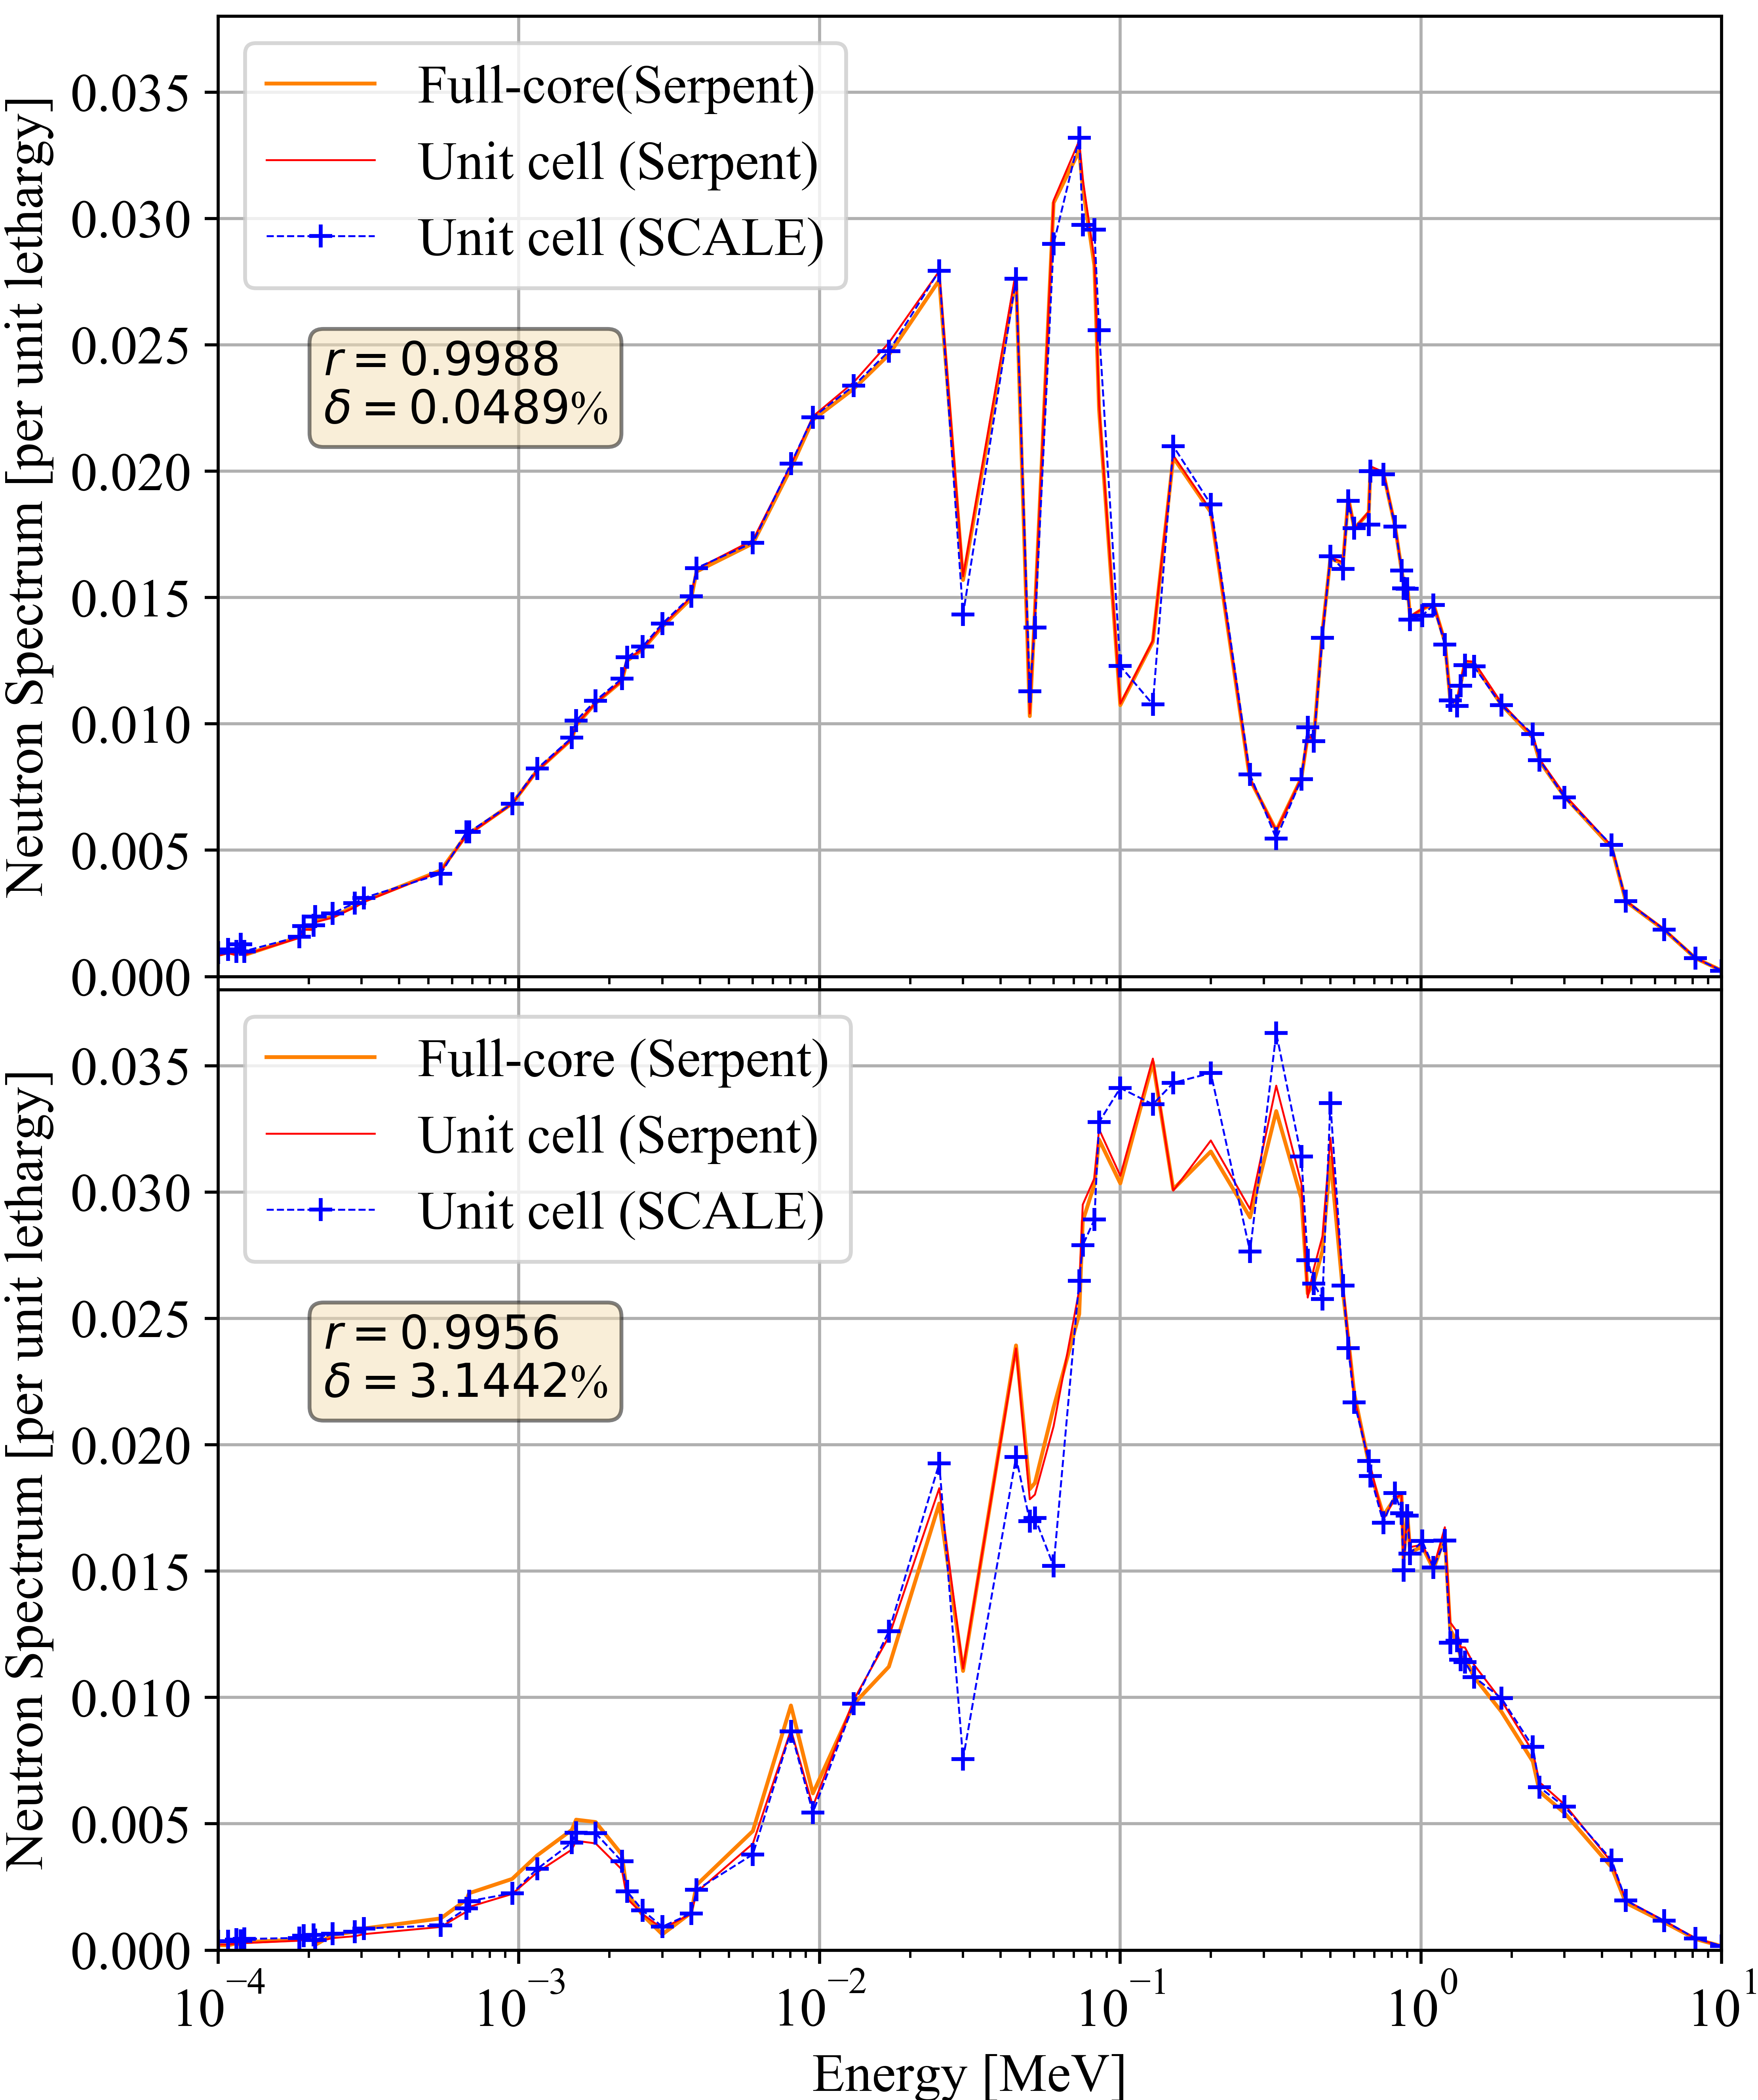
\includegraphics[width=0.65\textwidth]{./Figures/two_full_vs_unit_spectrum.png}
   \vspace{-0.05in}
  \caption{Neutron flux energy spectrum for full-core and unit cell models for two-fluid \gls{MSFR} (top) and \gls{MCSFR} (bottom).}
  \label{fig:spectrum_two}
    \vspace{-0.45in}
\end{figure}
\begin{figure}[!htb]
  \centering
  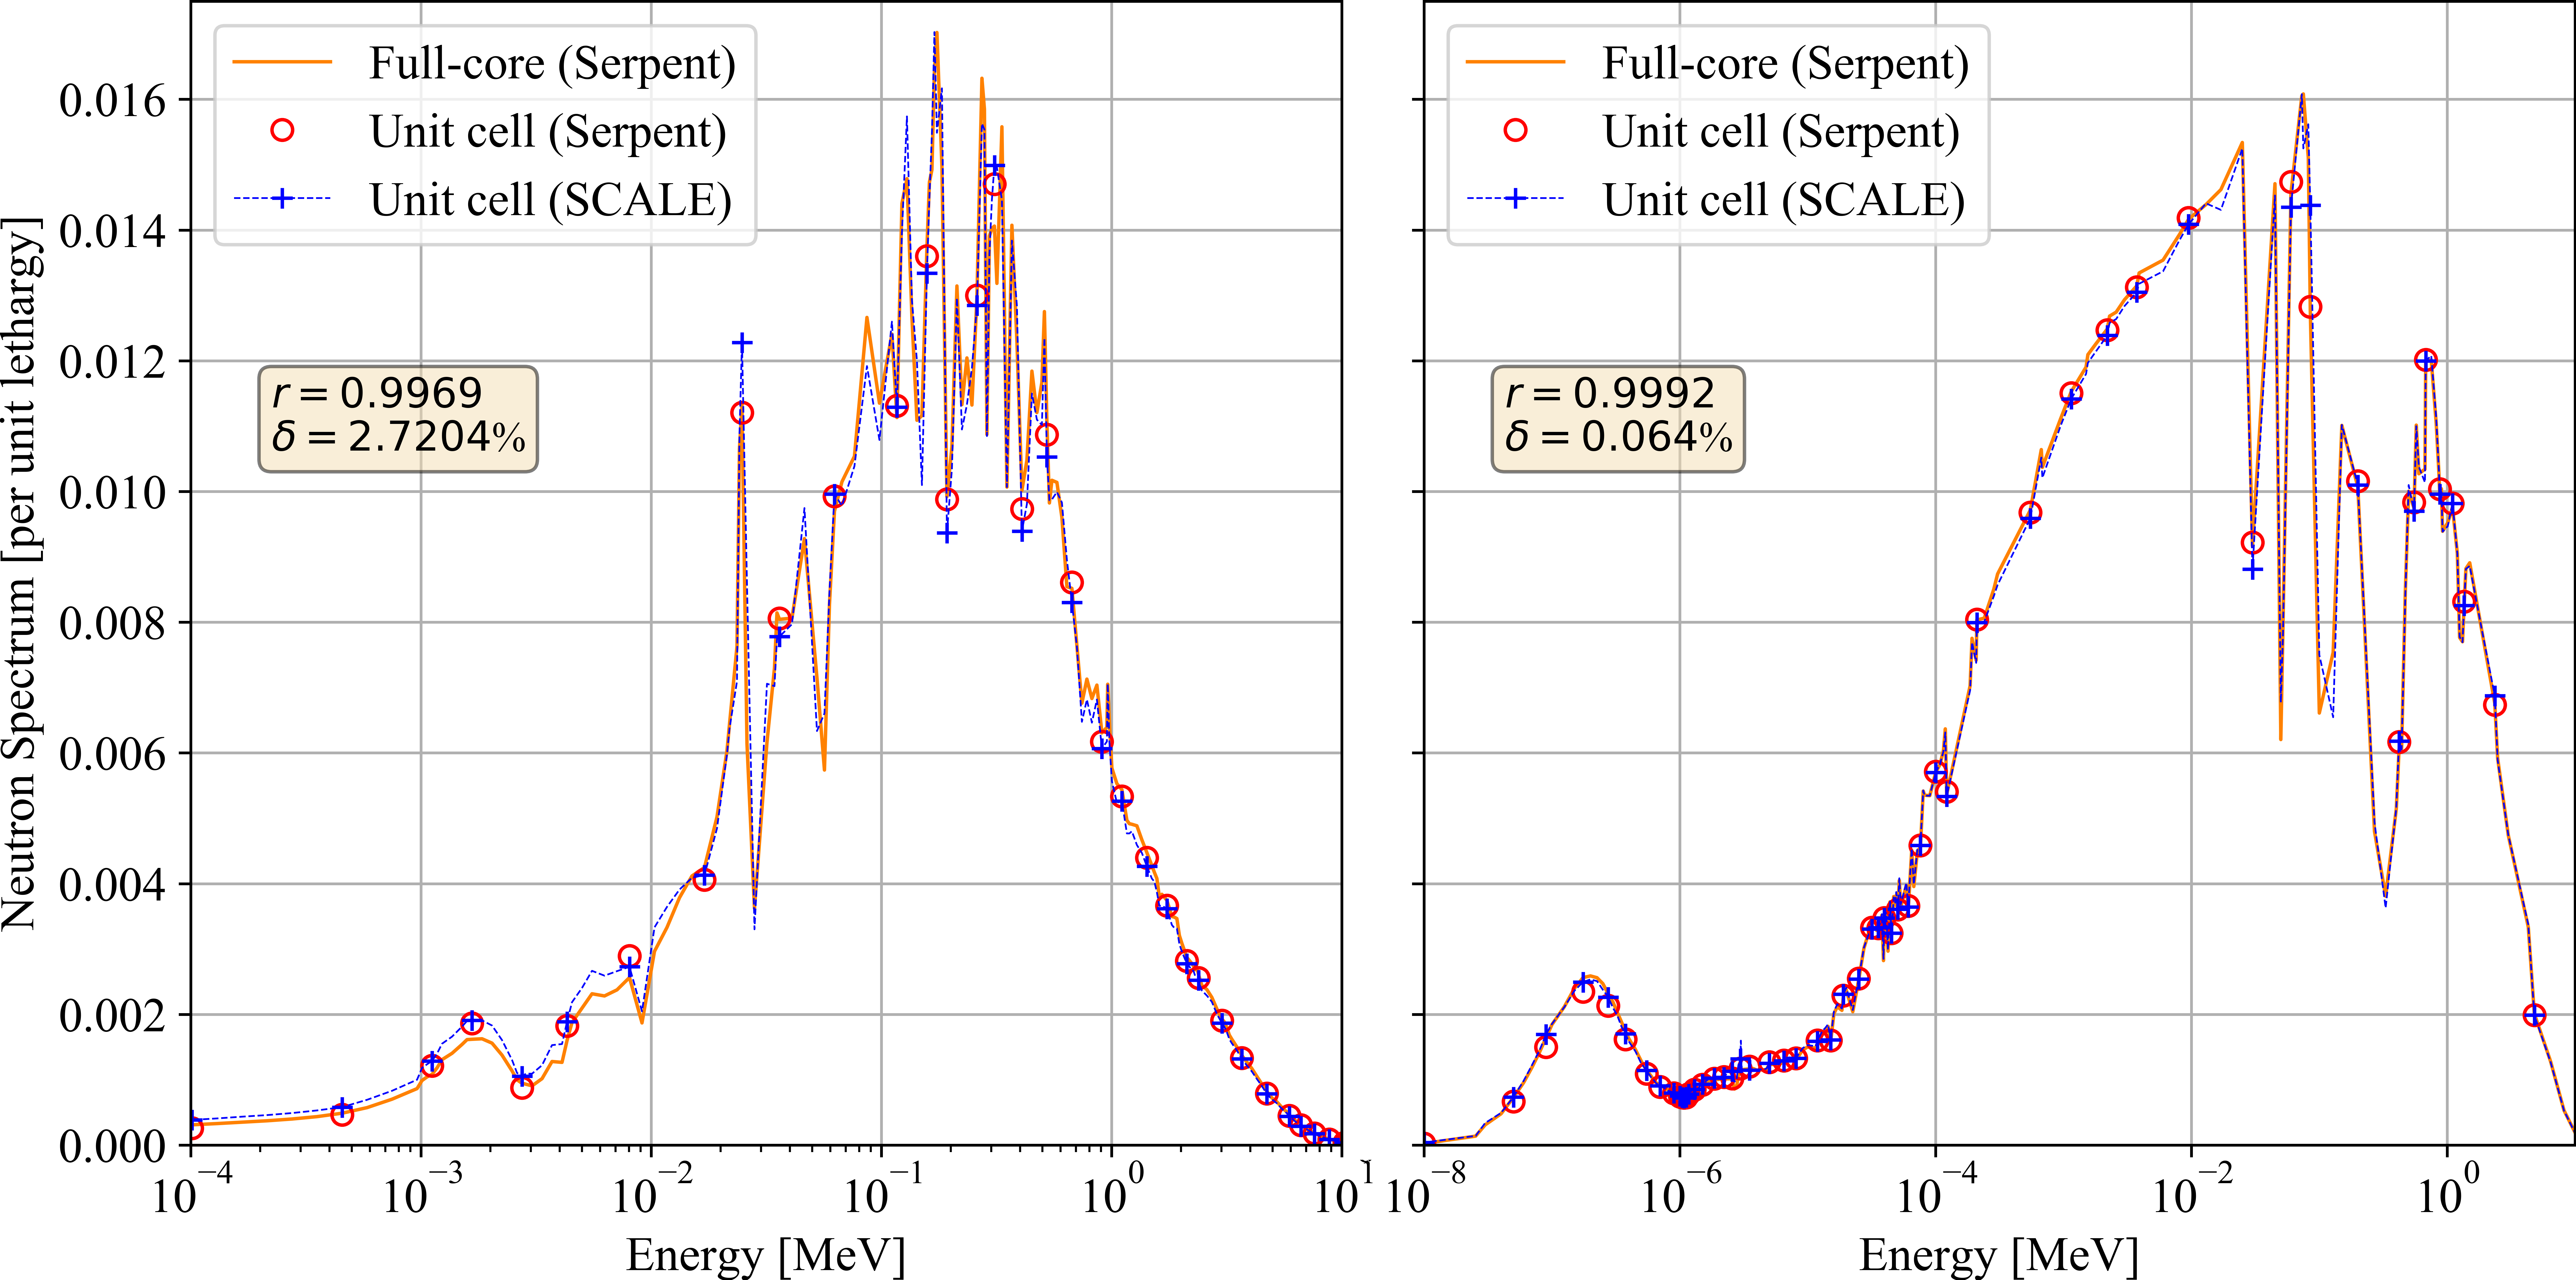
\includegraphics[width=\textwidth]{./Figures/rebus_mosart_spectrum.png}
  	  \vspace{-0.2in}
  \caption{Neutron flux energy spectrum for full-core and unit cell models for single-fluid REBUS-3700 (left) and \gls{MOSART} (right).}
  \label{fig:spectrum_rebus}
    \vspace{-0.45in}
\end{figure}
%\begin{figure}[!htb]
%  \centering
%  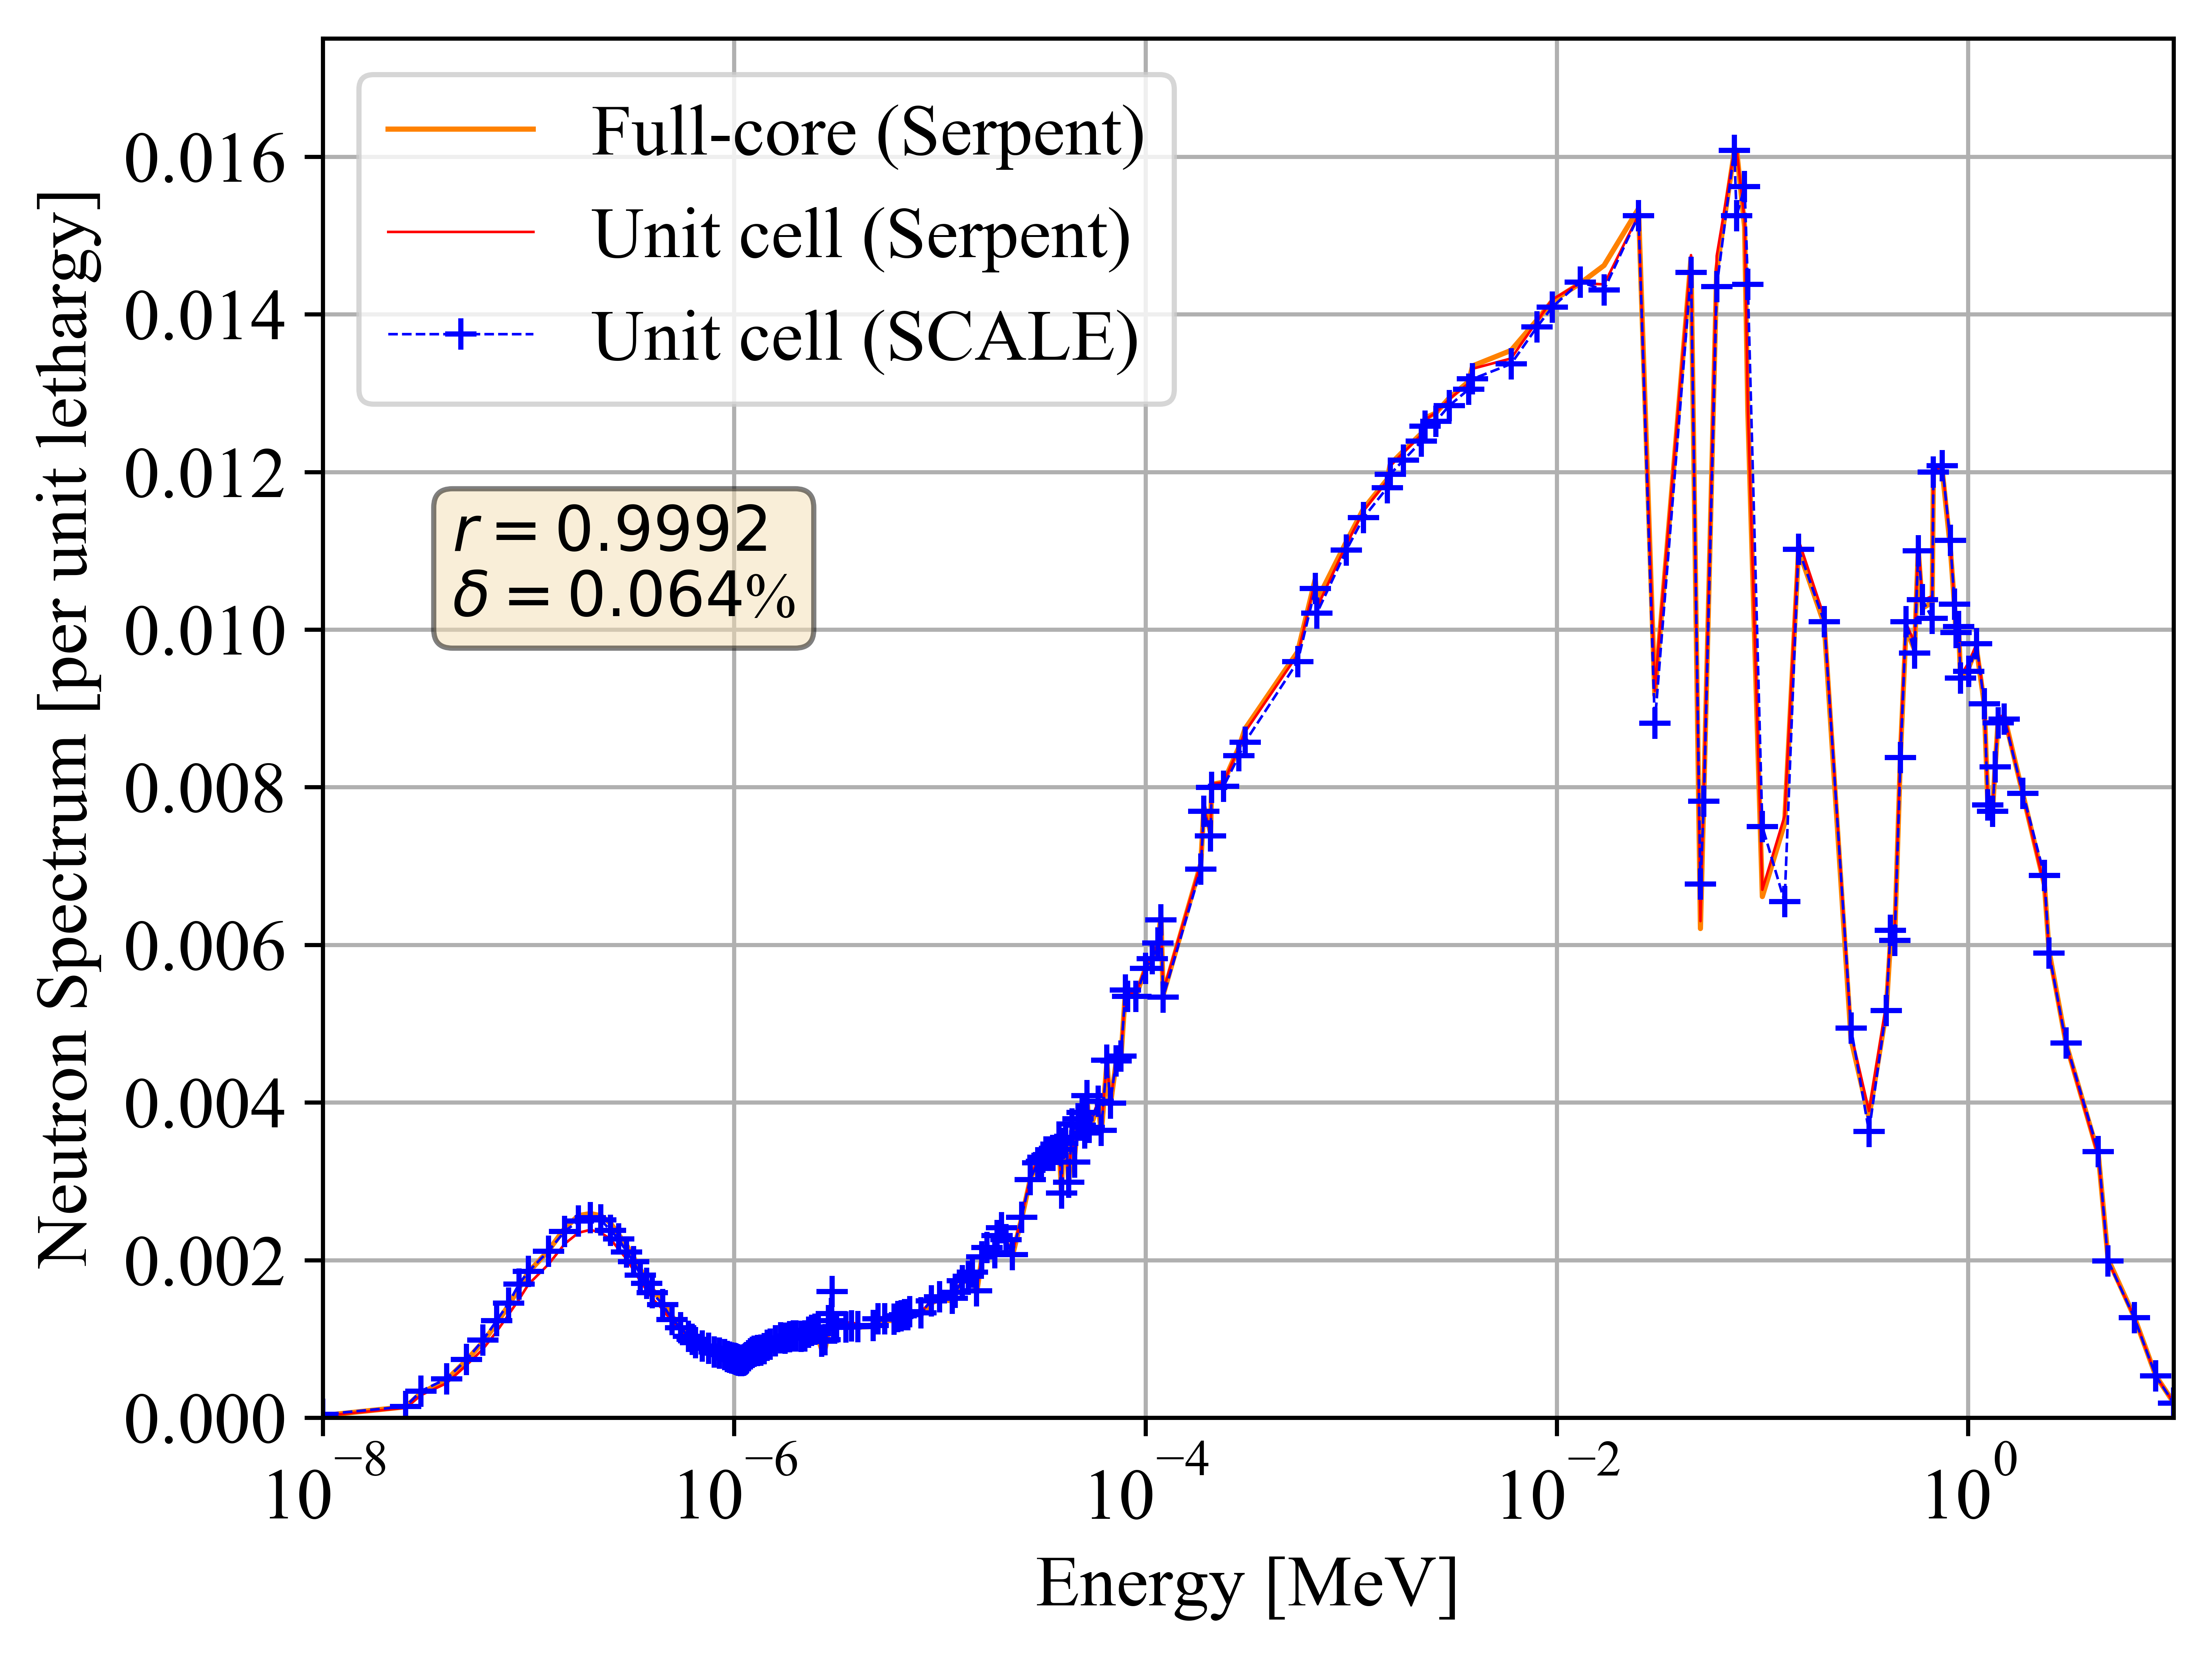
\includegraphics[width=0.7\textwidth]{./Figures/mosart_full_vs_unit_spectrum.png}
%  	  \vspace{-0.1in}
%  \caption{Neutron flux energy spectrum for full-core and unit cell models for single-fluid \gls{MOSART} with graphite reflector.}
%  \label{fig:spectrum_mosart}
%    \vspace{-0.25in}
%\end{figure}
\begin{figure}[!htb]
  \centering
  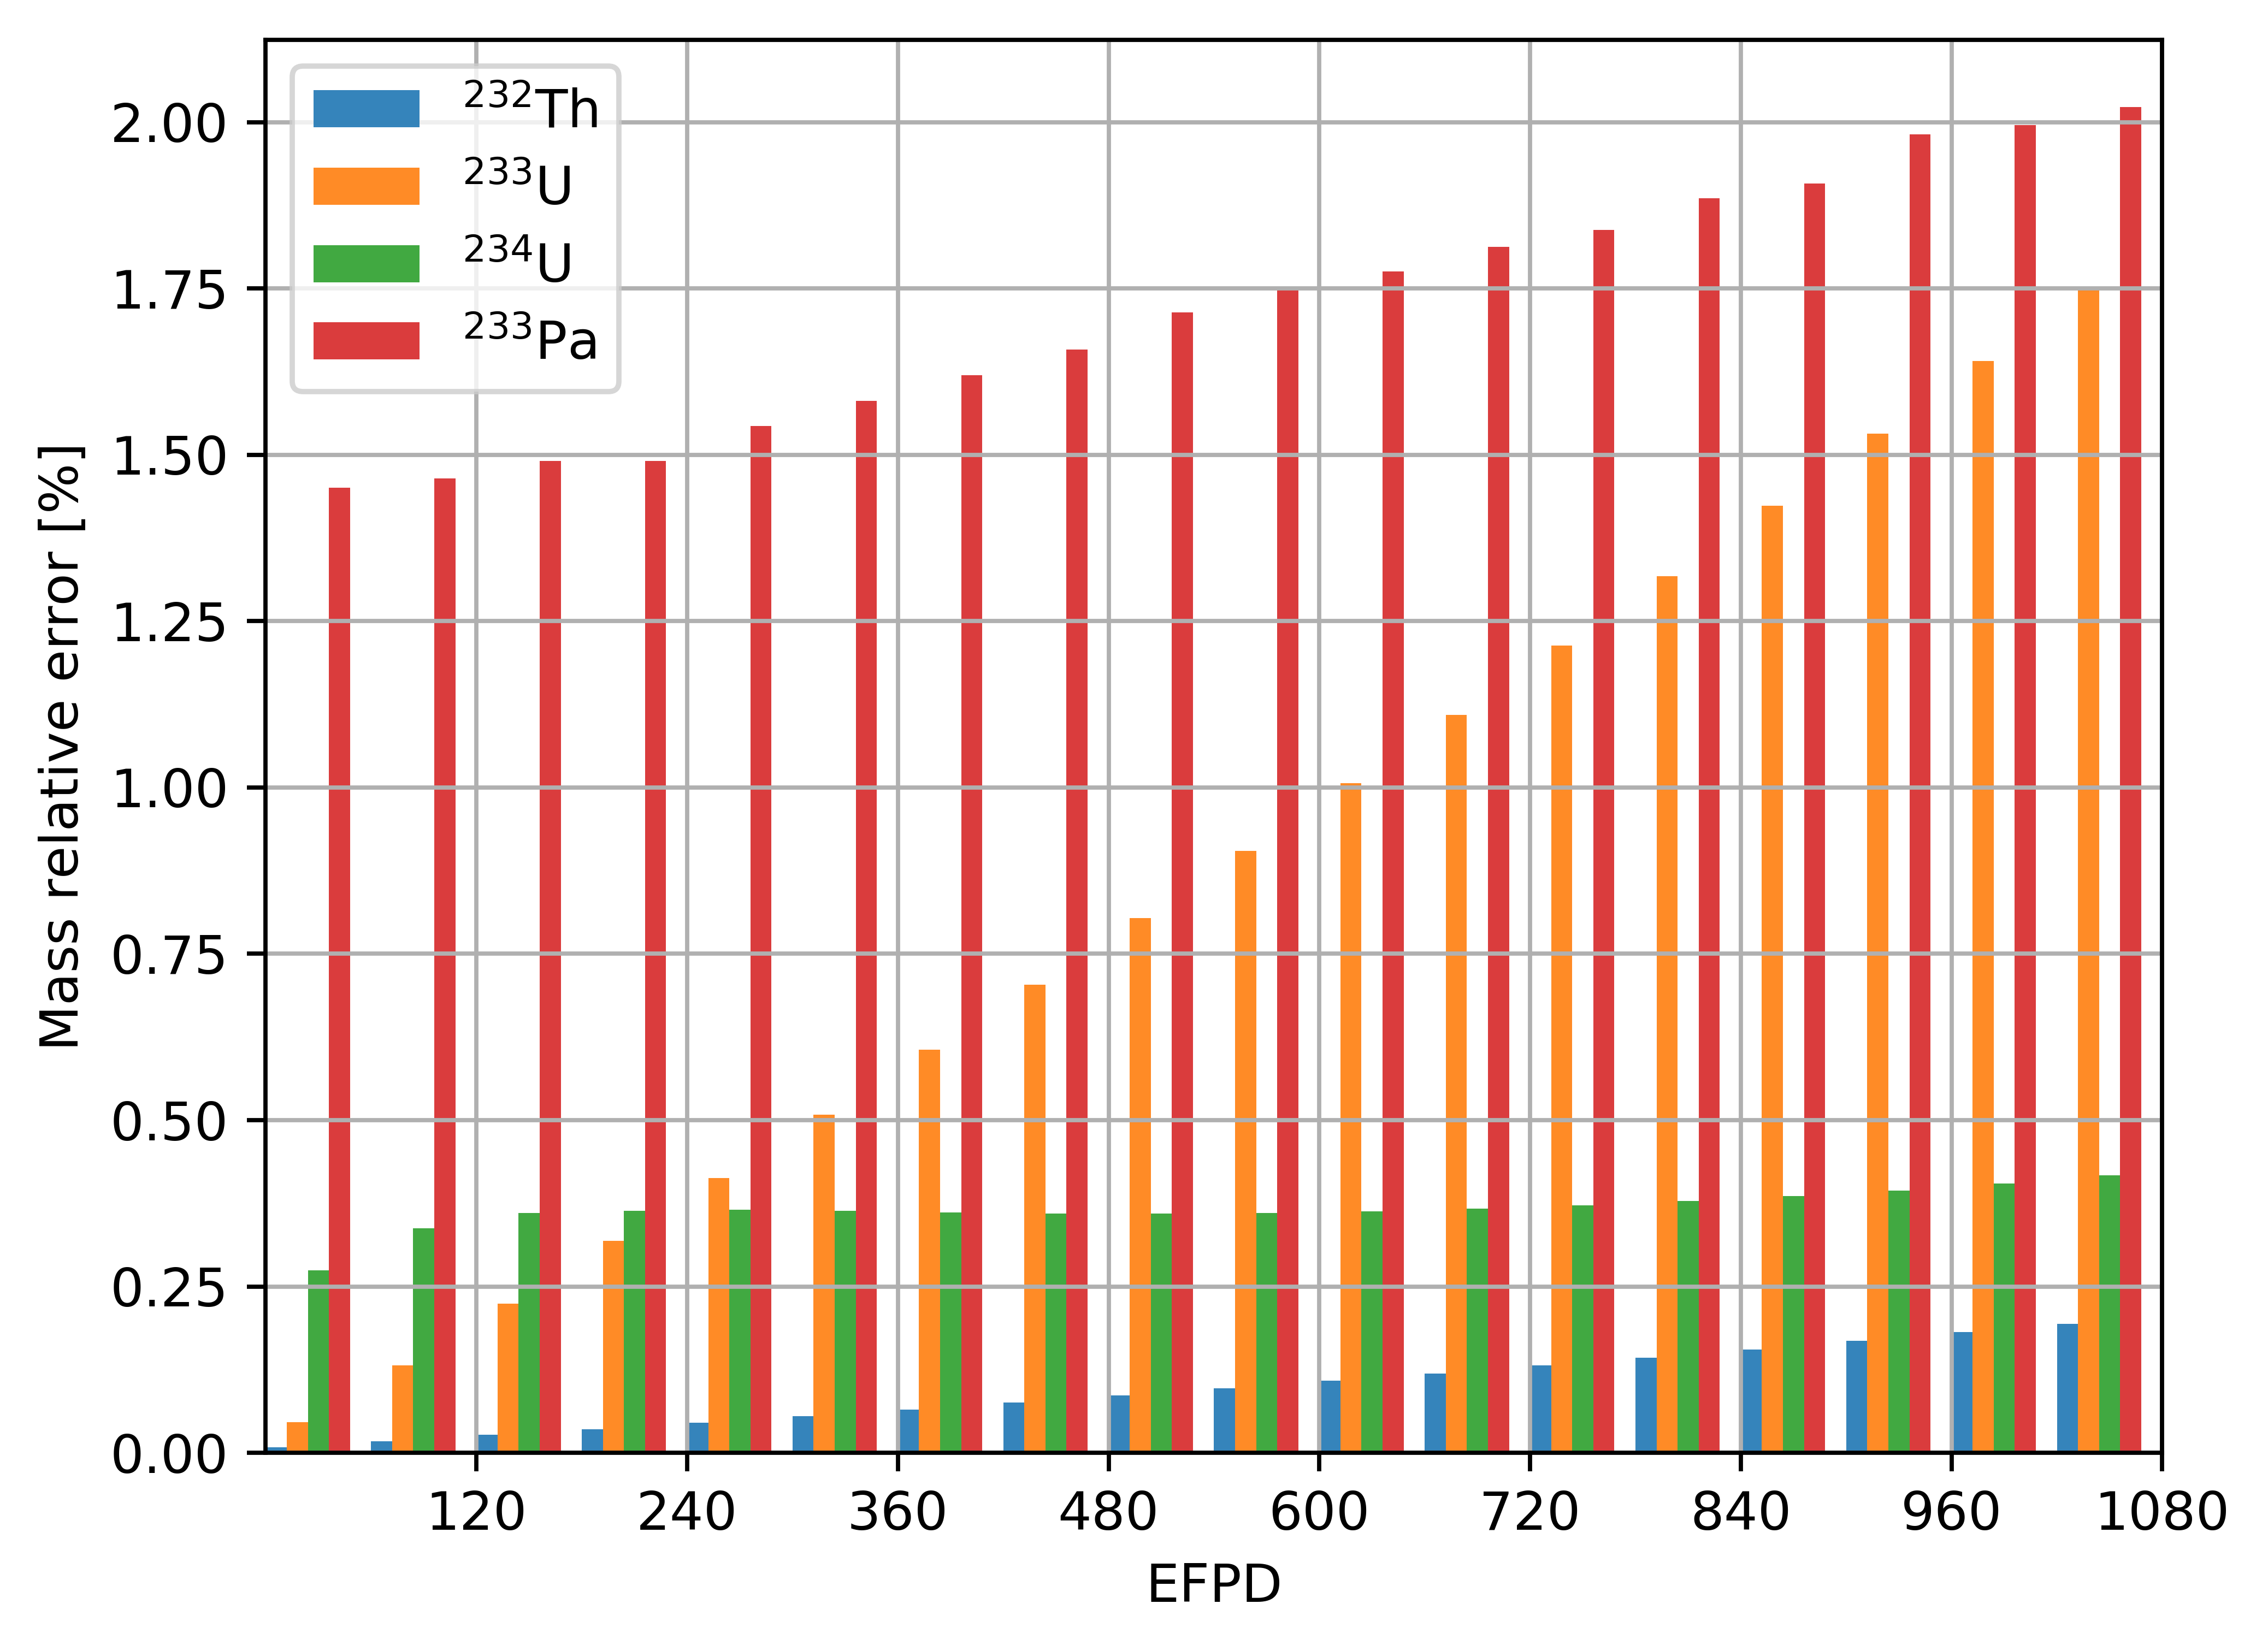
\includegraphics[width=0.7\textwidth]{./Figures/msfr_depl_f_vs_u.png}
  	  \vspace{-0.1in}
  \caption{Geometry approximation error in depleted mass of selected isotopes for the \gls{MSFR} during 1140 EFPD of operation without online reprocessing. Full-core and unit cell depletion using SERPENT2 (36 and 4 mln neutron histories, respectively).}
  \label{fig:msfr_depl_err}
    \vspace{-0.4in}
\end{figure}
For all four reactor concepts, the neutron energy spectra obtained with the SERPENT Monte Carlo and SCALE/TRITON agree very well as in previous studies \cite{betzler_fuel_2018}. Larger differences are observed in the intermediate energy ranges due to cross section resonances for these energies and to the limited number of energy groups for SCALE/TRITON. Continuous-energy physics is expected to provide better results as it does not suffer from inaccurate cross section representations in resonances and the fast energy range. 

Finally, the unit cell approximation accuracy for depletion simulations was estimated using SERPENT2 burnup capabilities for the full-core and unit cell model of the \gls{MSFR} (\Cref{fig:msfr_depl_err}). This plot demonstrates that relative error of geometry approximation for important isotopes mass after 1140 EFPD (Effective Full-Power Day) of salt irradiation is less than 2\% and increasing during operation. The error grows because of statistical uncertainty accumulation due to the nature of the Monte Carlo method. Furthermore, the unit cell approximation has provided a \textbf{20x} speedup over the original full-core model.

Overall, the unit cell approximation is quite accurate for fast \gls{MSR}s but further method optimization (e.g., using problem-oriented cross section libraries optimized for fast reactors) needed to achieve better accuracy.
\subsection{Fuel cycle performance analysis}
\label{sec:performance}
\Cref{fig:k_inf} demonstrates that all reactors started with the same small excess of reactivity ($\approx$2000 pcm) and remained critical throughout the 60-year operational lifetime. The thorium-fueled \gls{MSFR} and \gls{MOSART} show a significant reactivity drop during the first few years of operation due to $^{233}$Pa accumulation; it is a strong neutron poison which $\beta$ decays to $^{233}$U with a half-life 27.4 days. For U/Pu concepts (\gls{MCSFR} and REBUS), $^{239}$Np $\beta$ decays \footnote{$^{238}$U captures a neutron to form $^{239}$U which almost immediately $\beta$ decays to $^{239}$Np} to $^{239}$Pu much faster ($\tau_{1/2}=2.356$ days). Therefore, a lower fissile material feed rate is needed to compensate this breeding delay.

\Cref{fig:msfr-u-balance,fig:mosart-balance} shows heavy metals inventory evolution for four selected fast \gls{MSR} designs during 60 years of operation on 100\% power level. Two-fluid \gls{MSFR} breeds $^{233}$U from $^{232}$Th in the driver (core) and in the blanket. Fissile material produced in the blanket is continuously removed and then rerouted in two directions: (1) to the driver to compensate fuel burnup and maintain the reactor criticality; (2) to fissile material storage. Notably, a significant amount of $^{234}$U was accumulated in the core and significantly deteriorates breeding performance because $^{234}$U is a neutron poison. Thus, to avoid this parasitic absorption, $^{233}$Pu (which is a precursor for $^{234}$U production) should be isolated from the core in a separate tank where protactinium decays to $^{233}$U. This approach was suggested by \gls{ORNL} for thermal \gls{MSBR} concept \cite{robertson_conceptual_1971} and can be employed for fast \gls{MSR}s too.

Similarly, the \gls{MCSFR} breeds $^{239}$Pu from $^{238}$U and directly produces a considerable amount of non-fissile $^{240}$Pu. The $^{240}$Pu has high absorption cross section which degrades the neutron economy. The \gls{MCSFR} at the end of 60-year operation cycle has about 28 t of fissile $^{239}$Pu left in the storage and driver, and demonstrate the best among four considered designs doubling time, 17 years (e.g., during 60 years of operation the \gls{MCSFR} produces enough $^{239}$Pu to startup $\approx3.5$ additional reactors of this type).

Single-fluid \gls{MOSART} is operated as a quite efficient \gls{LWR} \gls{SNF} transmuter (\Cref{fig:mosart-balance}). TRU from spent fuel is used as a fissile material (similarly to \gls{MOX} fuel for \gls{LWR}s) to breed new fissile $^{233}$U from $^{232}$Th. Notably, \gls{MOSART} has graphite reflector to shift the neutron spectrum to the  intermediate range (\Cref{fig:spectrum_rebus}) because $^{233}$U breeding is more efficient in the thermal neutron energy range. Moreover, total TRU inventory increases  during operation to compensate for parasitic neutron poisoning (poisoning by $^{240}$Pu, $^{234}$U, etc). Overall, \gls{MOSART} over 60 years of operation consumed 43.68 t of TRU from \gls{LWR} \gls{SNF}, 26.7 t of $^{232}$Th, while produced 66.4 GWe-yr and has 2.3 t of fissile $^{233}$U left in the core at the end of the lifetime.

Similarly to the \gls{MOSART}, REBUS-3700 also uses TRU from \gls{LWR} as a fuel but operates in $^{238}$U/$^{239}$Pu fuel cycle. This fast \gls{MSR} concept maintained  TRU and natural uranium inventory almost constant over 60 years without any issues related to neutron poisons accumulation. It is possible due to the very hard neutron spectrum of this \gls{MSR} concept (\Cref{fig:spectrum_rebus}). Notably, REBUS-3700 does not need continuous fissile material feed (only fertile material feed), over 60 years of operation REBUS-3700 consumed 85 t of natural uranium, 18 t of TRU as start-up fuel, while produced 102 GWe-yr and has 10.5 t of fissile $^{239}$Pu inventory at the end of the lifetime. 
\begin{figure}[!htb]
  \centering
  \vspace{-0.3in}
  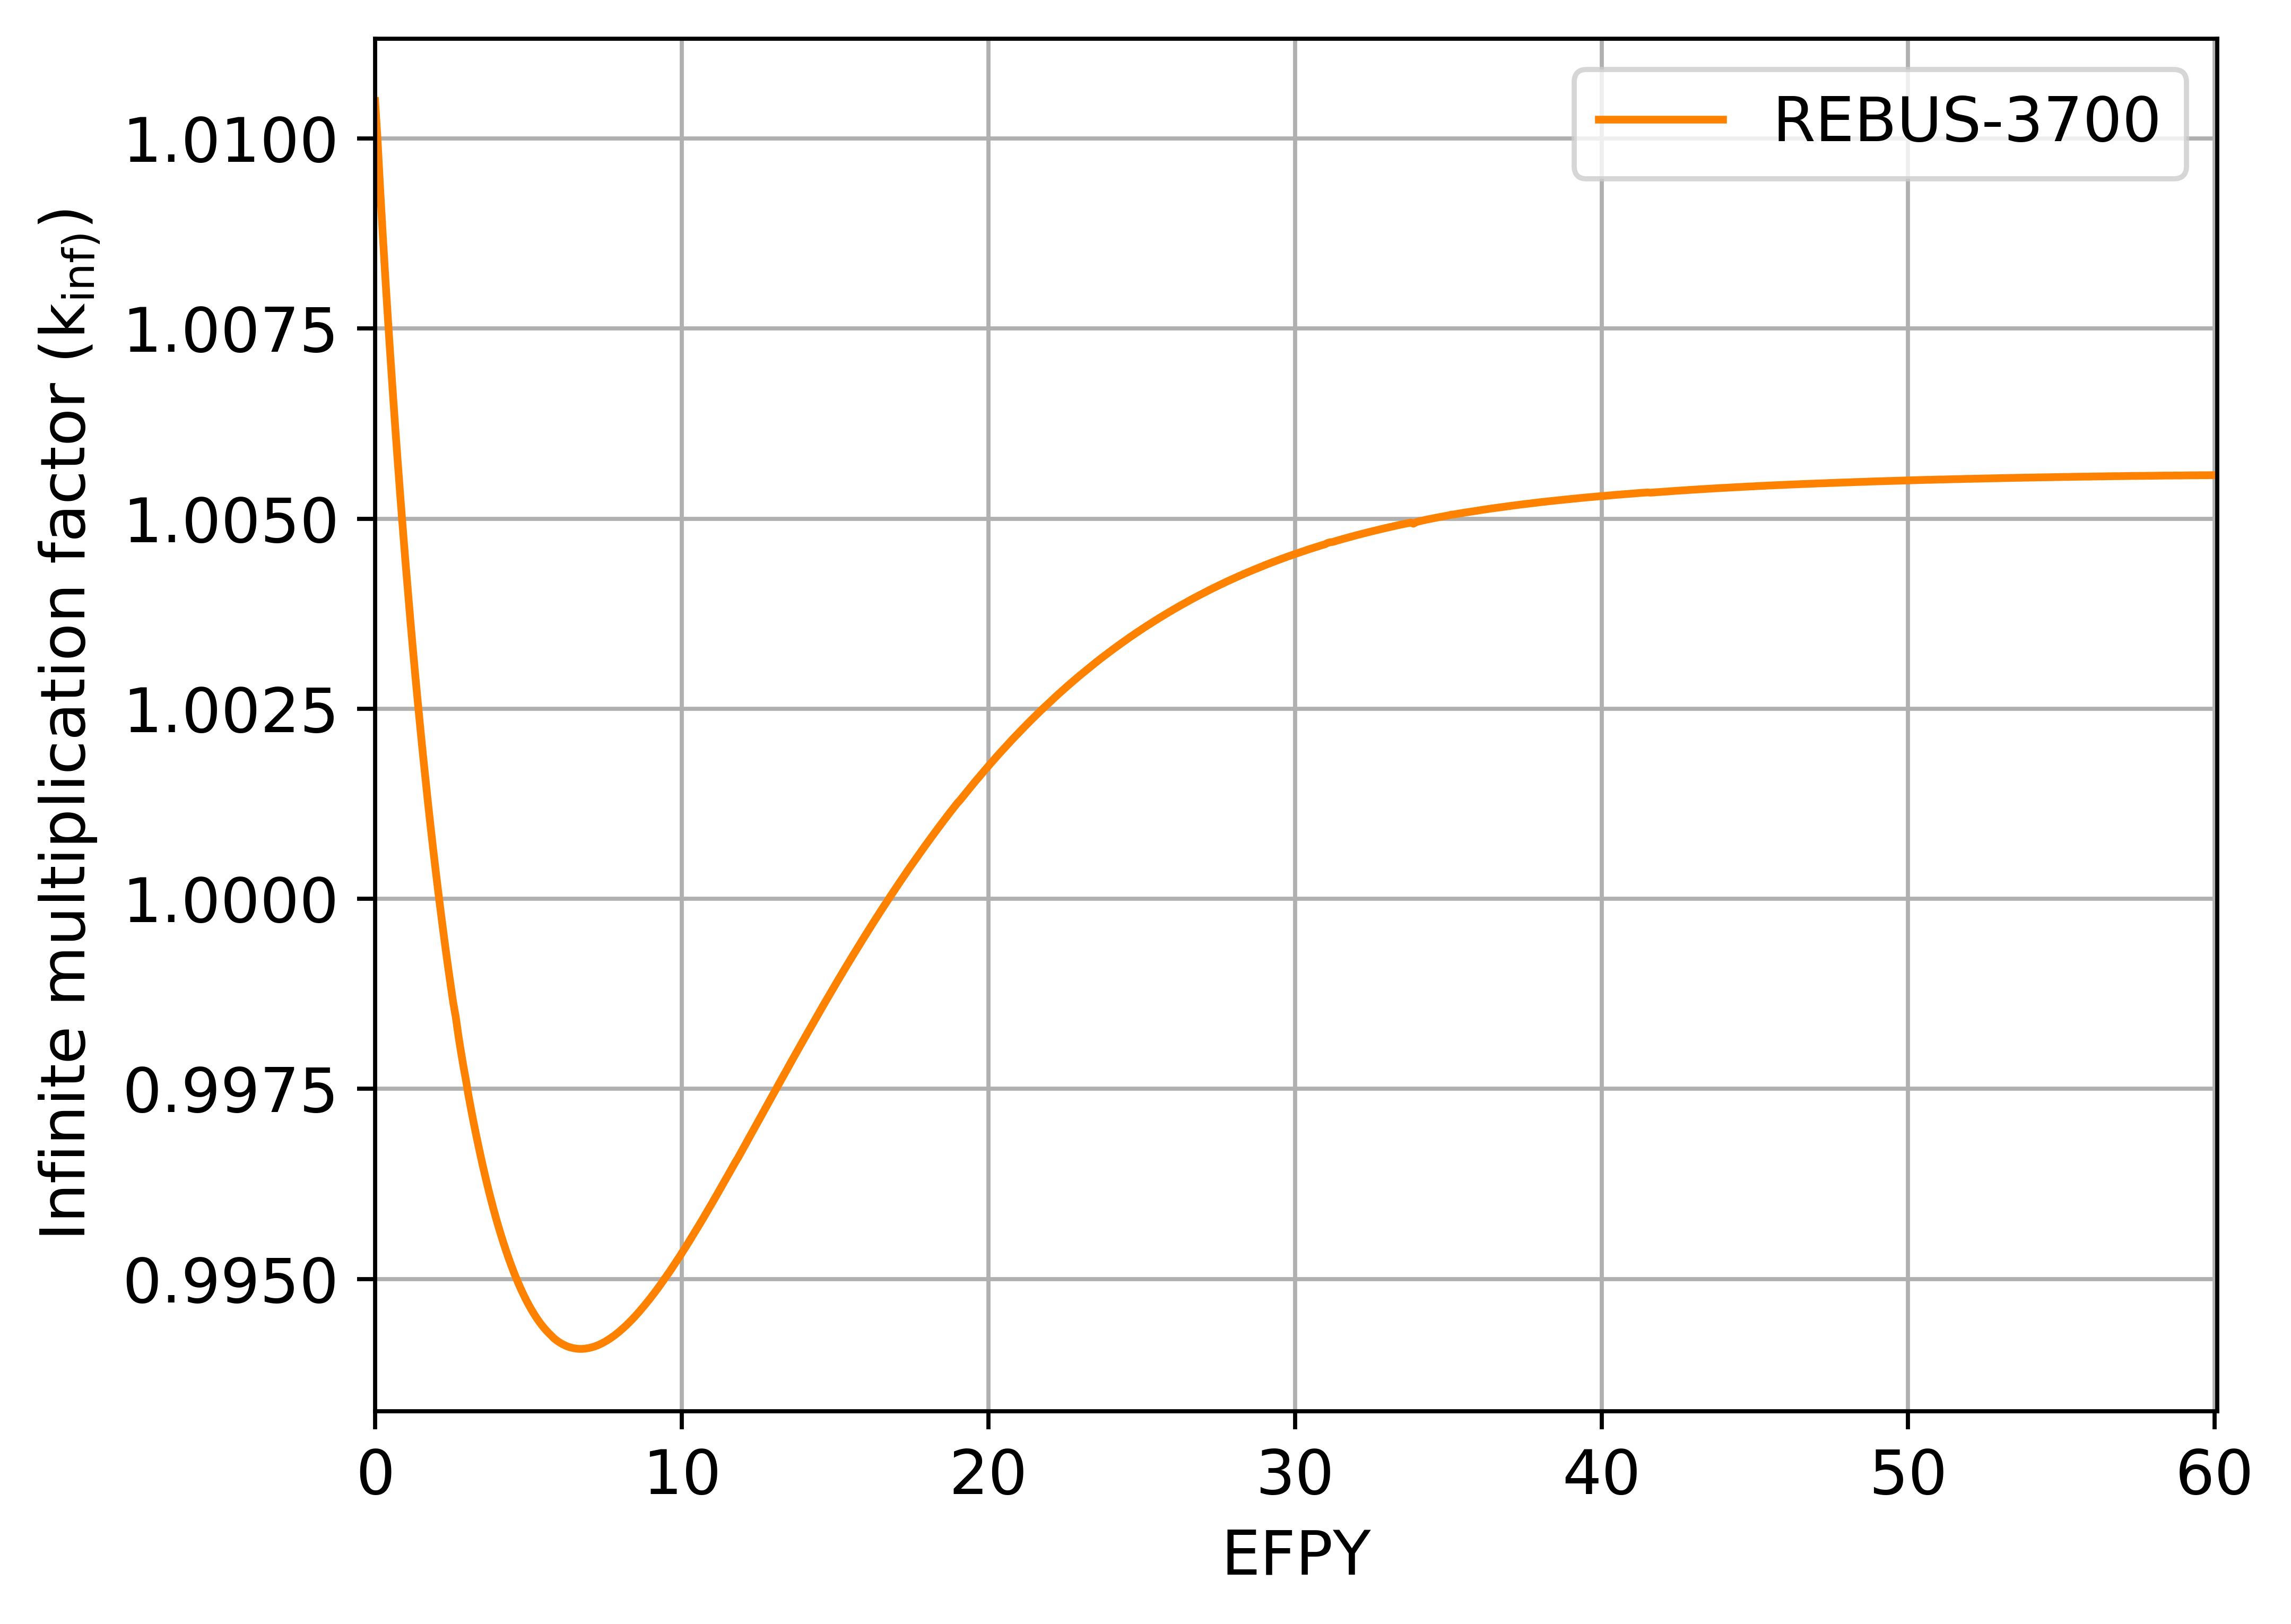
\includegraphics[width=0.65\textwidth]{./Figures/k_inf.png}
	  \vspace{-0.15in}
  \caption{Infinite multiplication factor for four reactor designs during 60 years of operation.}
  \label{fig:k_inf}
    \vspace{-0.4in}
\end{figure}
\begin{figure}[!htb]
  \centering
  \includegraphics[width=\textwidth]{./Figures/msfr_mcsfr_balance.png}
	  \vspace{-0.2in}
  \caption{\gls{MSFR} (left) and \gls{MCSFR} (right) heavy metal isotopic salt content during operation calculated with the unit cell model (238-group transport).}
  \label{fig:msfr-u-balance}
    \vspace{-0.5in}
\end{figure}
\begin{figure}[!htb]
  \centering
  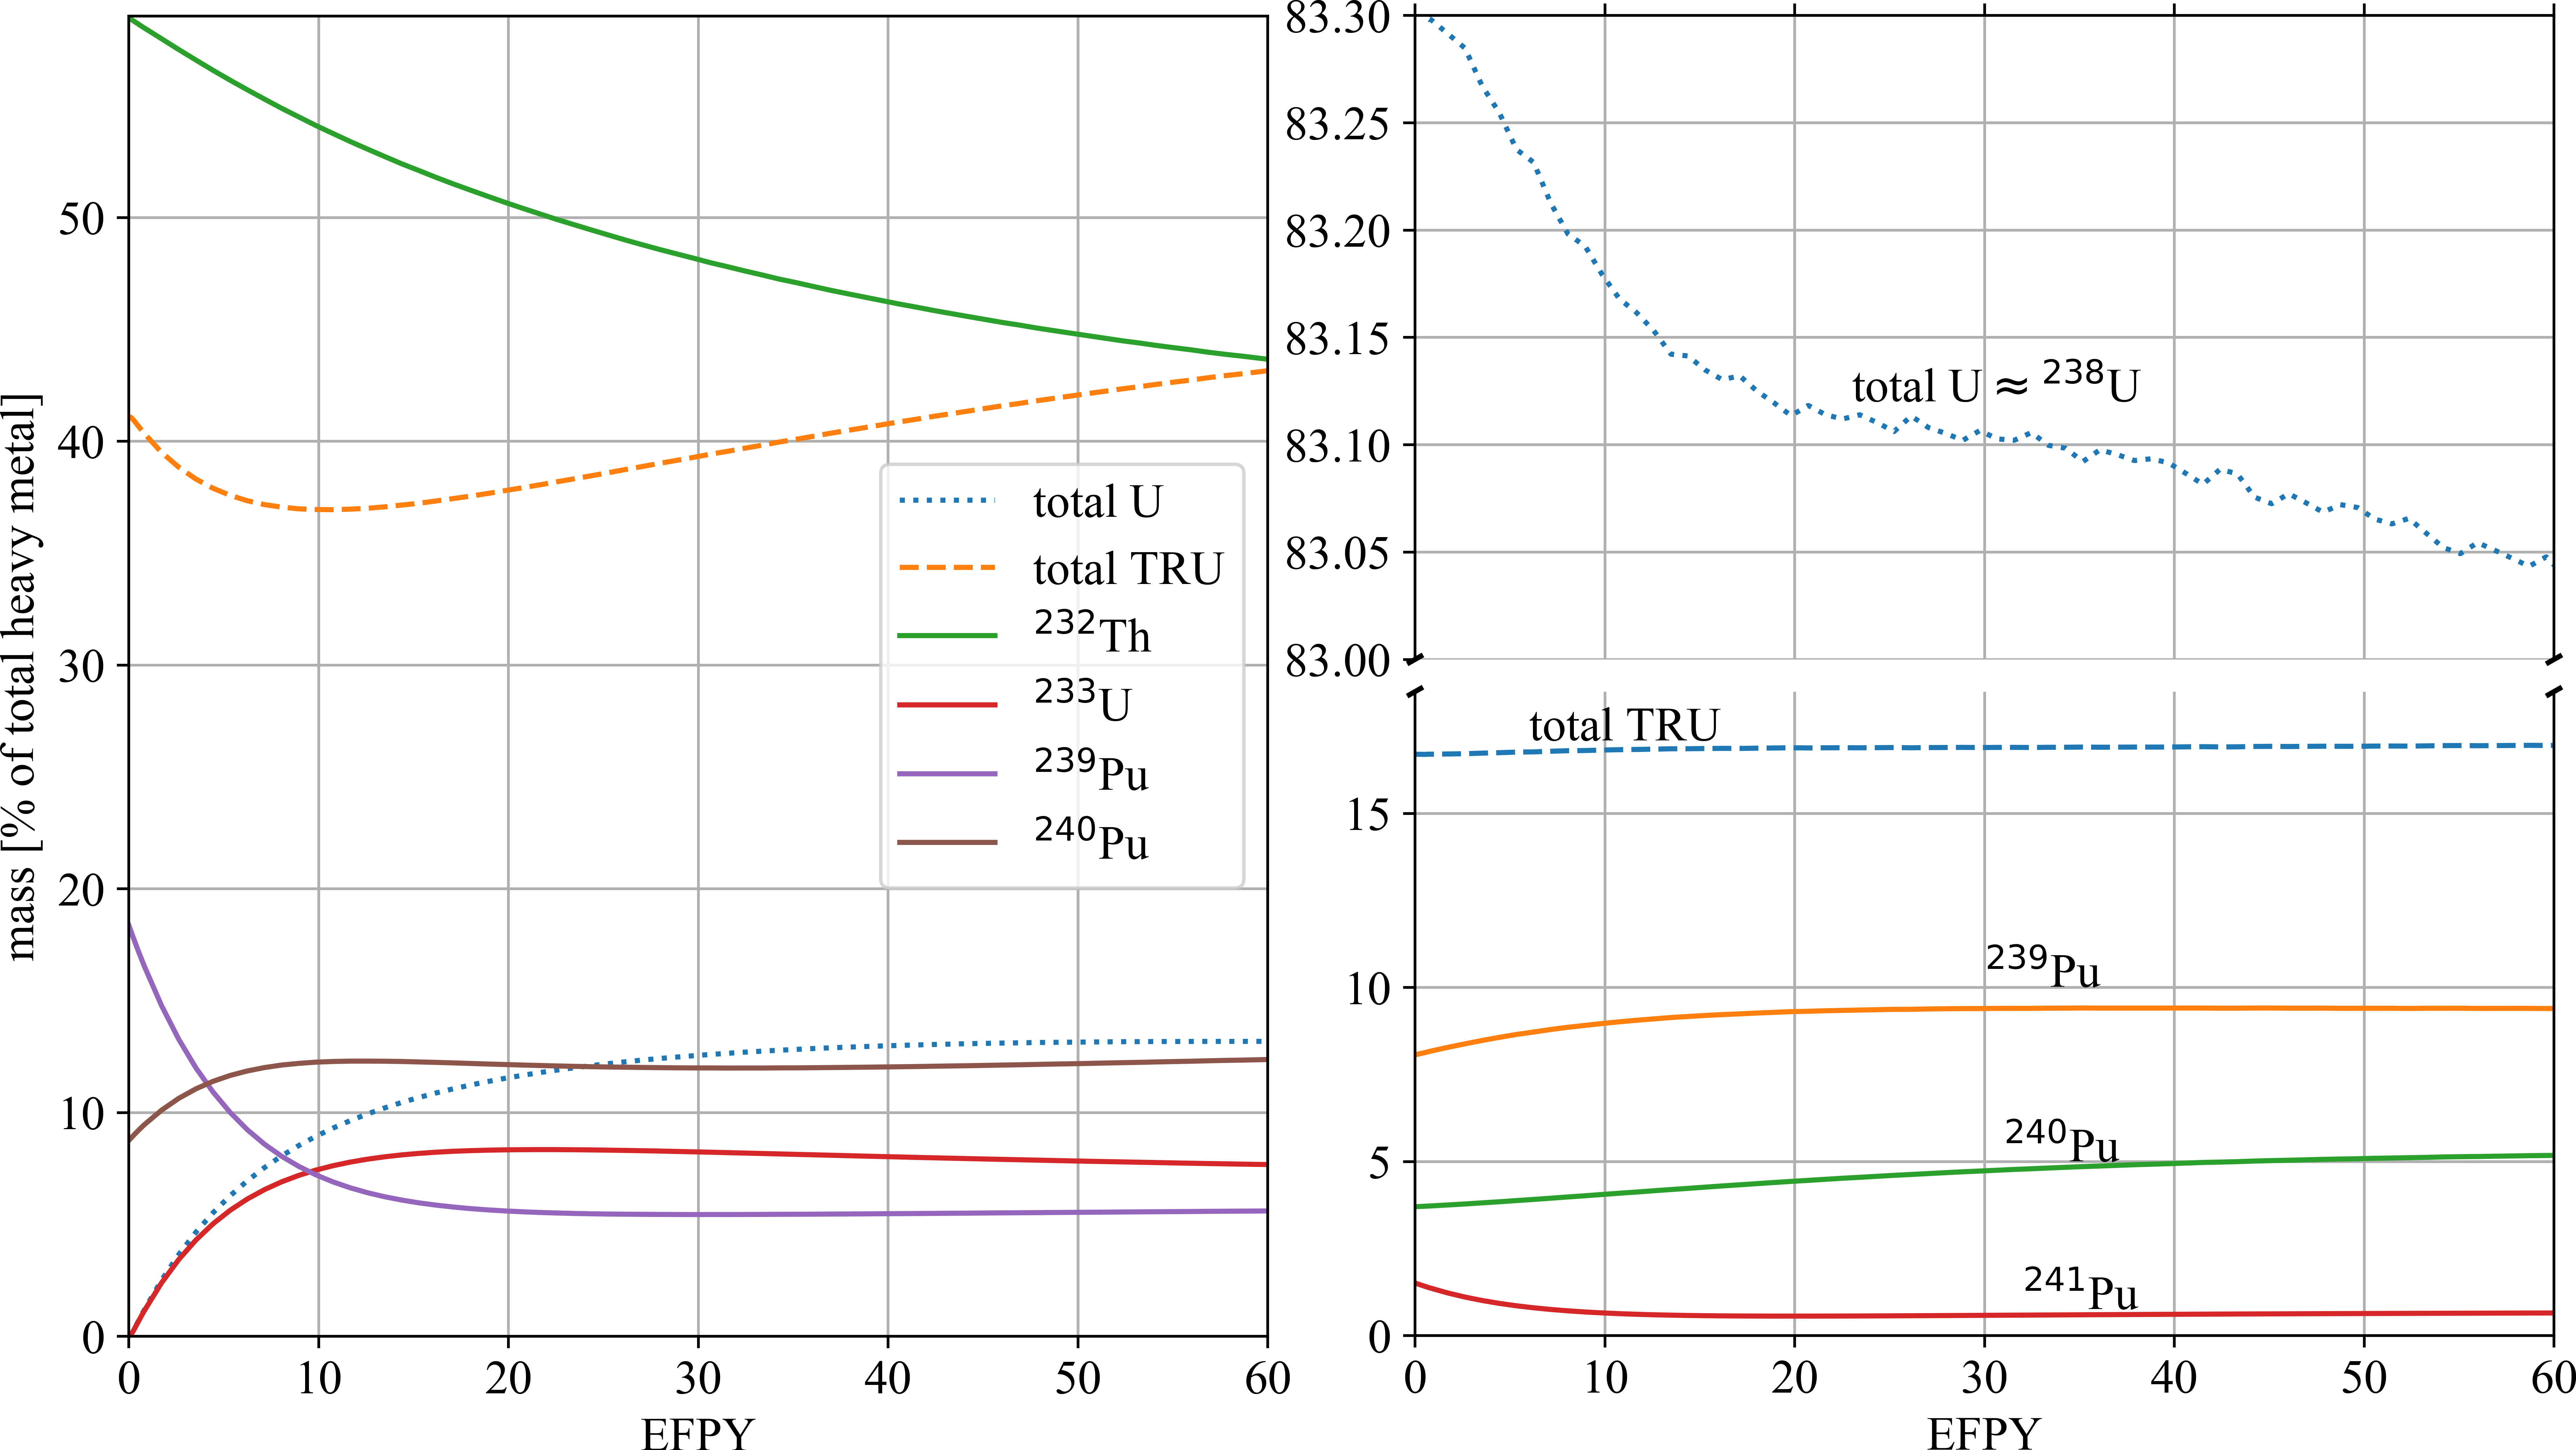
\includegraphics[width=\textwidth]{./Figures/mosart_rebus_balance.png}
  	  \vspace{-0.2in}
  \caption{\gls{MOSART} (left) and REBUS-3700 (right) heavy metal isotopic salt content during operation calculated with the unit cell model (238-group transport).}
  \label{fig:mosart-balance}
    \vspace{-0.3in}
\end{figure}
\subsection{E\&S Evaluation Metrics}
\label{sec:metrics}
Evaluation Metrics were calculated using E\&S guide \cite{wigeland_nuclear_2014-4} to evaluate fast \glspl{MSR} fuel cycle performance and compare it with other perspective designs (table~\ref{table:metrics}). Normalized per GWe-yr, the \gls{MOSART} and \gls{MSFR} concepts required only 0.402 and 0.663 t of natural thorium, respectively. Natural uranium utilization per energy generated for the U/Pu cycle concepts \gls{MCSFR} and REBUS is less than 0.9 t/GWe-yr. None of the considered reactor designs disposed of heavy metals (\gls{DU}+\gls{RU}+\gls{RTh}) as these were operated in continuous recycle fuel cycles.
\begin{table*}[hb!]
  \vspace{-0.5in}
  \centering
  \caption{The E\&S Evaluation Metrics of selected fast spectrum \gls{MSR} designs.}
  \label{table:metrics}
  \begin{tabular}{p{0.48\textwidth} p{0.1\textwidth} p{0.1\textwidth} p{0.1\textwidth} p{0.1\textwidth}} \toprule
   Parameter &  \gls{MSFR} & \gls{MCSFR} & REBUS & \gls{MOSART} \\ \midrule
   Evaluation Group	&  EG28 & EG23 & EG24 & EG28   \\
   Natural Uranium or Thorium Utilization, t/GWe-yr & 0.663(Th) & 0.973 (U) & 0.834 (U) & 0.402(Th) \\
   Mass of \gls{SNF}+\gls{HLW} disposed, t/GWe-yr & 0.866 & 0.894 & 0.813 &  0.820 \\
   Mass of DU+RU+RTh disposed, t/GWe-yr & 0.0 & 0.0 & 0.0 &  0.0 \\
   Products from Reprocessing/Separation technology, t: \gls{RU}/\gls{RTh}/\gls{TRU}/\gls{FP} &
   8.7/41.9/ 0.36/69.51 &  83.2/0.0/ 32.8/140.3 & 92.6/0/ 18.9/79.6 & 3.9/12.9/ 12.9/54.1  \\
 \bottomrule
  \end{tabular}
    \vspace{-0.4in}
\end{table*}

Low natural resources consumption results in a total waste reduction (\gls{SNF}+\gls{HLW}) to less than 0.9 t/GWe-yr comparing with 21.92 t/GWe-yr for conventional \gls{LWR} and 9.22 t/GWe-yr for advanced \gls{HTGR} \cite{wigeland_nuclear_2014-4}. 
In addition, \gls{MOSART} and REBUS both use \gls{TRU} separated from \glspl{LWR} \gls{SNF} as fissile material. It may be helpful to reuse \gls{SNF} from 60 years of nuclear power generation. Notably, the lower natural resources utilization do not directly correlate with the mass of disposed waste because TRU from \gls{LWR} \gls{SNF} to fuel the \gls{MOSART} and REBUS was considered as ``free" resource and was not included in natural uranium/thorium mass. Overall, the considered \gls{MSR} designs outperform competitive fuel cycle technologies (EG23, EG24, EG28) for resource utilization and waste generation but $^{233}$U/Th fast critical reactors with continuous recycle and new enriched uranium as startup fuel (EG27, EG37) presumably would perform even better.
\section{CONCLUSIONS}
The fuel cycle performance of four fast spectrum \gls{MSR} designs was analyzed to determine key fuel cycle metrics. Full-core SERPENTS Monte Carlo code and unit cell SCALE/TRITON transport models were created to prove the viability of using simplified unit cell models for long-term (i.e., 60 years) depletion simulations to reduce computational burdens. Comparison between full-core and unit cell fluxes shows a relative error of less than 3.2\% and a correlation coefficient of 0.9956, while the unit cell geometry approximation has provided a 20x speedup.

Unit cell depletion simulations with continuous fission product removal and constant fertile/fissile material feeds show that with a startup infinite multiplication factor of about 1.02, all concepts remain critical during 60 years of operation. Natural uranium or thorium utilization varies from 0.402 t/GWe-yr for the thorium-fueled \gls{MOSART} to 0.973 MTU/GWe-yr for the U/Pu \gls{MCSFR}. \gls{SNF}+\gls{HLW} generation normalized per GWe-yr for all four designs is much less than that for conventional \glspl{LWR}: 0.894 t for \gls{MCSFR}, 0.866 t for \gls{MSFR}, 0.813 t for REBUS-3700, and 0.82 t for \gls{MOSART}. Furthermore, natural resources utilization normalized per GWe-yr for considered \gls{MSR} designs is more effective comparing with ``representative" designs in the EST study: (EG23) 0.973 and 1.34 t for the \gls{MCSFR} and ``representative" U/Pu \gls{SFR}, respectively; (EG24) 0.834 and 1.37 t for the REBUS and TRU-fueled \gls{SFR}; (EG28) 0.402 and 1.68 t for the \gls{MOSART} and thorium-fueled \gls{SFR}.

Moreover, the \gls{MCSFR}, \gls{MOSART}, and REBUS designs produce a considerable amount of \gls{TRU}; some fissile material from this may be recovered from the salt after reactor shutdown and reused to start up additional reactors. Particularly, the amount of fissile material after the 60-year lifetime of the \gls{MCSFR} is enough to start up three additional units of this type; the amount of \gls{TRU} after the end of life of REBUS may be used for the initial core loading of one additional REBUS unit or two \gls{MOSART} units. 

The unit cell time-dependent analyses that were performed demonstrate predicted fuel cycle performance for fast spectrum \glspl{MSR} concepts and provide direction for future performance studies and design improvement. Additional validation of SCALE/TRITON Alpha against another continuous reprocessing code (e.g., SERPENT2) and/or batch-wise Python package SaltProc \cite{rykhlevskii_advanced_2018} is required to provide more confidence in the results.

Continued research into fast \glspl{MSR} topic could progress in a number of different directions. First and foremost, efforts should be made to simulate the \gls{MSFR} with additional protactinium isolation system which enhance $^{233}$U breeding for two perspective startup fissile compositions: (1) TRU to evaluate the \gls{MSFR} performance as a waste burner; (2) new enriched uranium because it promises better fuel cycle performance. Secondly, the \gls{MCSFR} design might be optimized to operate with startup composition based on enriched uranium instead of weapons-grade plutonium. Lastly, an additional area to explore is the accident safety analysis which requires the development of a multi-physics model of investigated fast \gls{MSR} designs with the coupled neutronics/thermal-hydraulics code, Moltres \cite{lindsay_introduction_2018}. The existing full-core SERPENT2 models and equilibrium fuel material compositions would be employed to generate problem-oriented nuclear data libraries for further usage
in accident transient analysis. 
%%%%%%%%%%%%%%%%%%%%%%%%%%%%%%%%%%%%%%%%%%%%%%%%%%%%%%%%%%%%%%%%%%%%%%%%%%%%%%%%
\section{Acknowledgments}
This research was supported by the DOE-NE Systems Analysis and Integration Campaign and by an appointment to the Oak Ridge National Laboratory Nuclear Engineering Science Laboratory Synthesis (NESLS) Program, sponsored by US Department of Energy and administered by the Oak Ridge Institute for Science and Education. Andrei Rykhlevskii and Prof. Kathryn Huff are also supported by DOE ARPA-E MEITNER program award DE-AR0000983.
%%%%%%%%%%%%%%%%%%%%%%%%%%%%%%%%%%%%%%%%%%%%%%%%%%%%%%%%%%%%%%%%%%%%%%%%%%%%%%%%
% You can enter a bibliography into the document using the following format, or use the
% bibliography style file "mandc.bst" found in the template directory.  You can use the bibliography style file
% by replacing the current bibliography block with:
\setlength{\baselineskip}{12pt}
\bibliographystyle{mandc}
\bibliography{2019-rykh-fsmsrs-mc}




\end{document}
